%\VignetteIndexEntry{genAriseGUI Vignette}
%\VignetteDepends{}
%\VignetteKeywords{microarray analyzer GUI}
%\VignettePackage{genAriseGUI}
\documentclass[12pt]{article}
\topmargin=0in
\oddsidemargin 0.0in
\evensidemargin 0.0in

\usepackage{Sweave}
\usepackage{graphicx}
\usepackage{fancyhdr}
\pagestyle{fancy}
\headheight 35pt 
\fancyhead[R]{\Large{\bf{genArise}}} %Especifico

\title{The genArise Package}
\author{Ana Patricia G\'omez May\'en\\ Gustavo Corral Guill\'e\\ Lina Riego\\ Gerardo Coello Couti\~no}

\begin{document}

\maketitle

\section{Introduction}

genArise is a package that contains specific functions to do the analysis of the obtained data of a microarray. You must install the packages tkrplot, tcltk and locfit in order to be able to use this package. genArise is loaded with the next instruction:\\
\begin{Schunk}
\begin{Sinput}
> library(genArise)
\end{Sinput}
\begin{Soutput}
Loading required package: locfit 
Locfit for R.
August 3, 2000.  (Updated for R 1.7.0, March 21, 2003)

Attaching package 'locfit':


	The following object(s) are masked from package:stats :

	 knots 

Loading required package: tkrplot 
Loading required package: tcltk 
\end{Soutput}
\end{Schunk}
Once loaded genArise, we can proceed with the analysis of the data of a microarray. genArise is provided of functions applied in an atomic way in every step of analysis, however there is a graphical user interface to facilitate the use of all the functions in the package. This graphic function will be described ahead, by now we will describe just the functions in a lower level.

\section{The Package's Functions}
The first that we must do is read the data contained in the input file. The format from the file must be columns of data separated by some character. The input file must contains only the rows with the data and no more, nevertheless it can have a header but this is not mandatory  to be able to read the files by the function.\\

To read the input files genArise contains the function \texttt{read.spot}. This function can read all data in the file, but it only consider the columns of interest for the analysis, in this case Cy3, Cy5, BgCy3, BgCy5 and the Ids.\\

This function returns an object of type Spot, and we will be working with this object. The syntax of this function is the next:

\begin{Scode}
> my.spot <- read.spot( file.name, cy3 = 1, cy5 = 2, 
  bg.cy3 = 3, bg.cy5 = 4, ids = 5, header = FALSE, 
  sep = "\t", is.ifc = FALSE)	
\end{Scode}

\begin{Soutput}
Output: an object of class Spot called my.spot
\end{Soutput}

In the input arguments of the function we must include the name of the input file and a number that indicates the position of the correspondig data in the file. The argument header indicates if the file contains header and the argument \texttt{is.ifc} represents a boolean that indicates if the file was done by the Microarray Unit of the Cellular Physiology Institute of UNAM. When this argument is TRUE, the columns without information of our interest will be ommited. So, when this argument is TRUE the other arguments (except the name of the input file) will be ignored. In this example, we suppose that the file just contains the columns of our interest. Besides, this columns are ordered.\\


Now exists an object of the class Spot in my.spot. This data corresponds to a fragment from a microarray of yeast that was done by the Microarray Unit of the Cellular Physiology Institute of UNAM. The original array has 24 grids, but this fragment corresponds only to the first two grids. We can define this object in the current environment in this way:

\begin{Schunk}
\begin{Sinput}
> data(Simon)
> ls()
\end{Sinput}
\begin{Soutput}
[1] "Simon"
\end{Soutput}
\end{Schunk}

\begin{Soutput}
We have created an object of the class Spot in the current
environment so we will be able to apply to that object any 
function of genArise that receives a spot as argument.
\end{Soutput}

In order to be able to visualize the data previous the analysis once we have read the input data, we can use the function \texttt{imageLimma()}. This function allows plot an image of colours representing the log intensity ratio for each  spot on the array and receives several arguments depending on the data that we are going to analyze.
\pagebreak

\begin{figure}[h]
\begin{center}
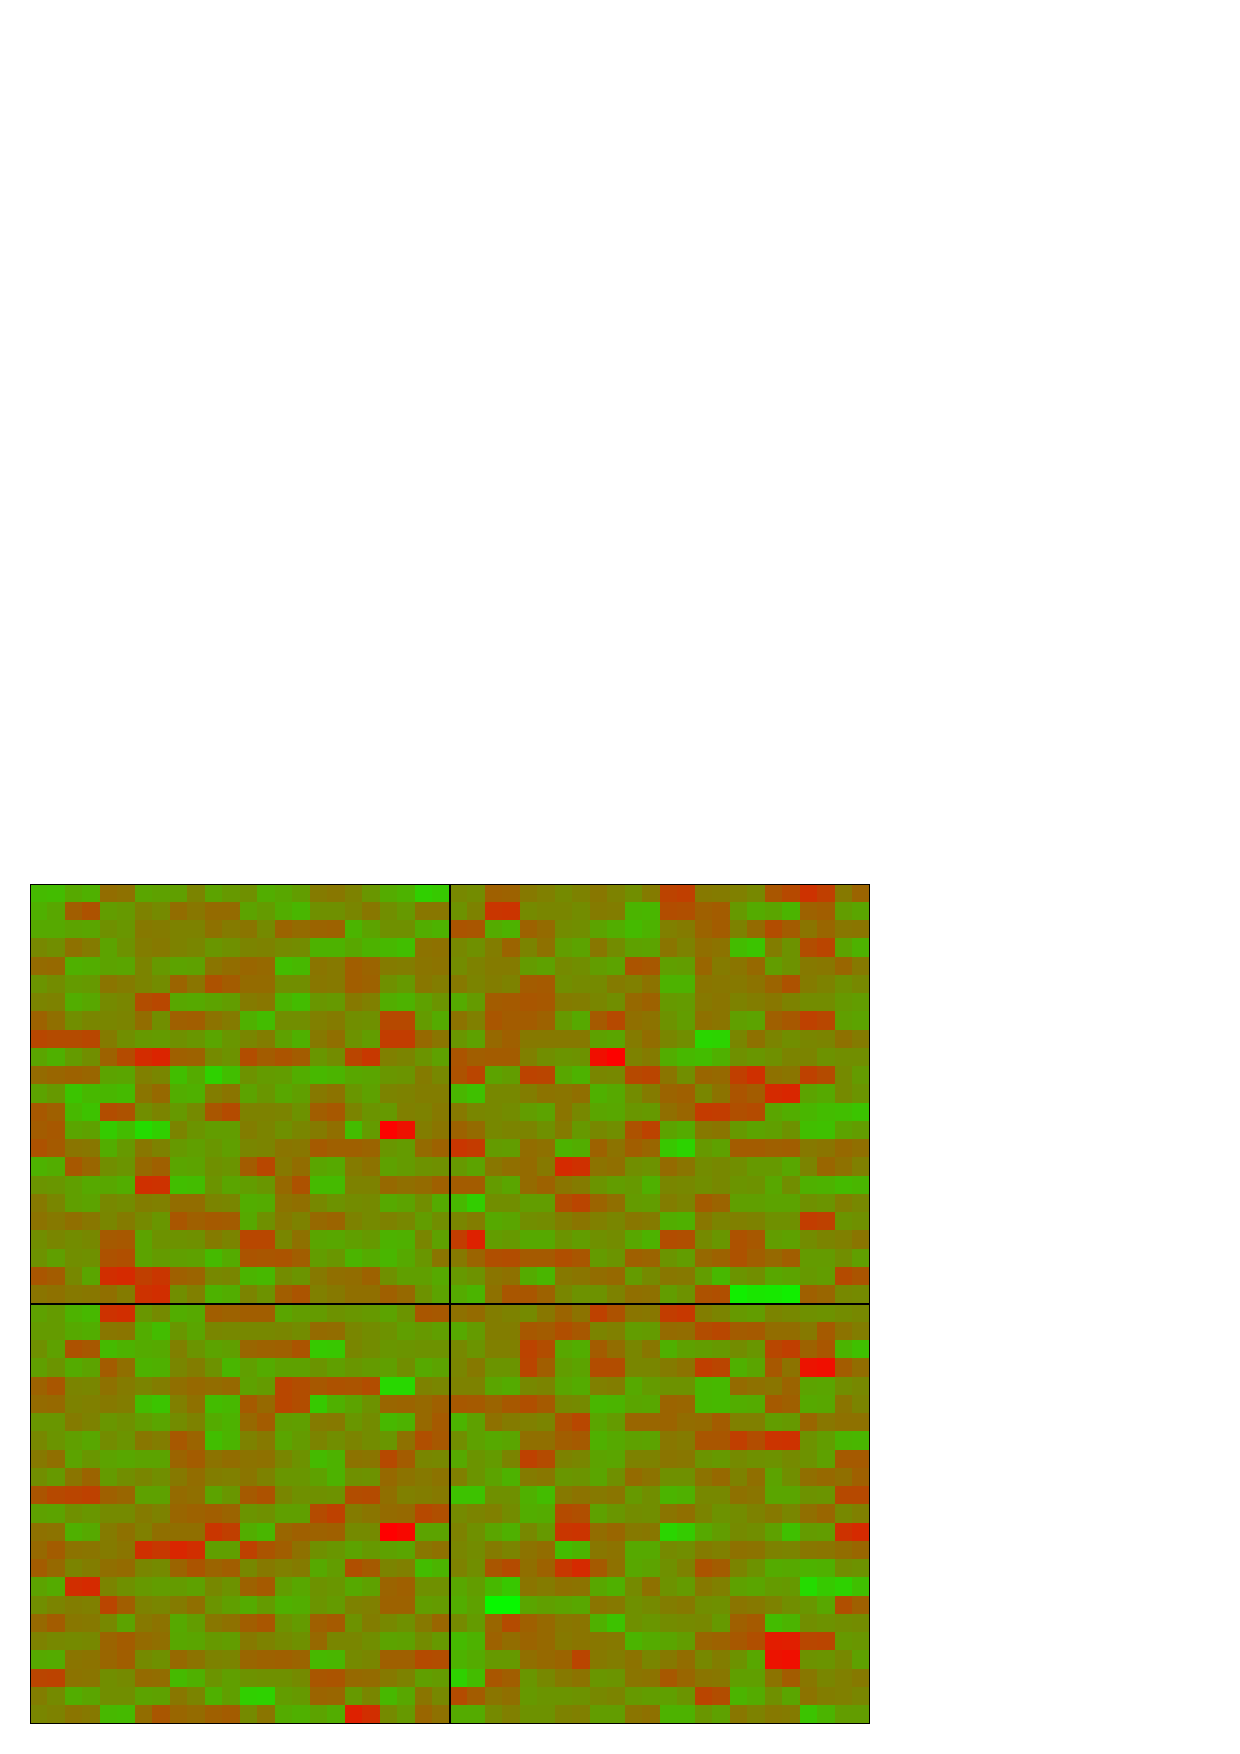
\includegraphics{example-genArise-003}
\caption{Cy3 and Cy5 intensities mixed.\label{fig1}}
\end{center}
\end{figure}
\begin{Scode}
> data(Simon)
> datos <- attr(Simon, "spotData")# Extract spot data
> M <- log(datos$Cy3, 2) - log(datos$Cy5, 2)
> imageLimma(z = M, row = 23, column = 24, meta.row = 2, 
  meta.column = 2, low = NULL, high = NULL)
\end{Scode}

\begin{Soutput}
Output: Plot the intensities values
\end{Soutput}

In the same way we can plot the values of each one of the intensities, this we can do it with the values of background corresponding to each one of the intensities.\\

For example, this is the plot for Cy3 intensities.
\begin{figure}[h]
\begin{center}
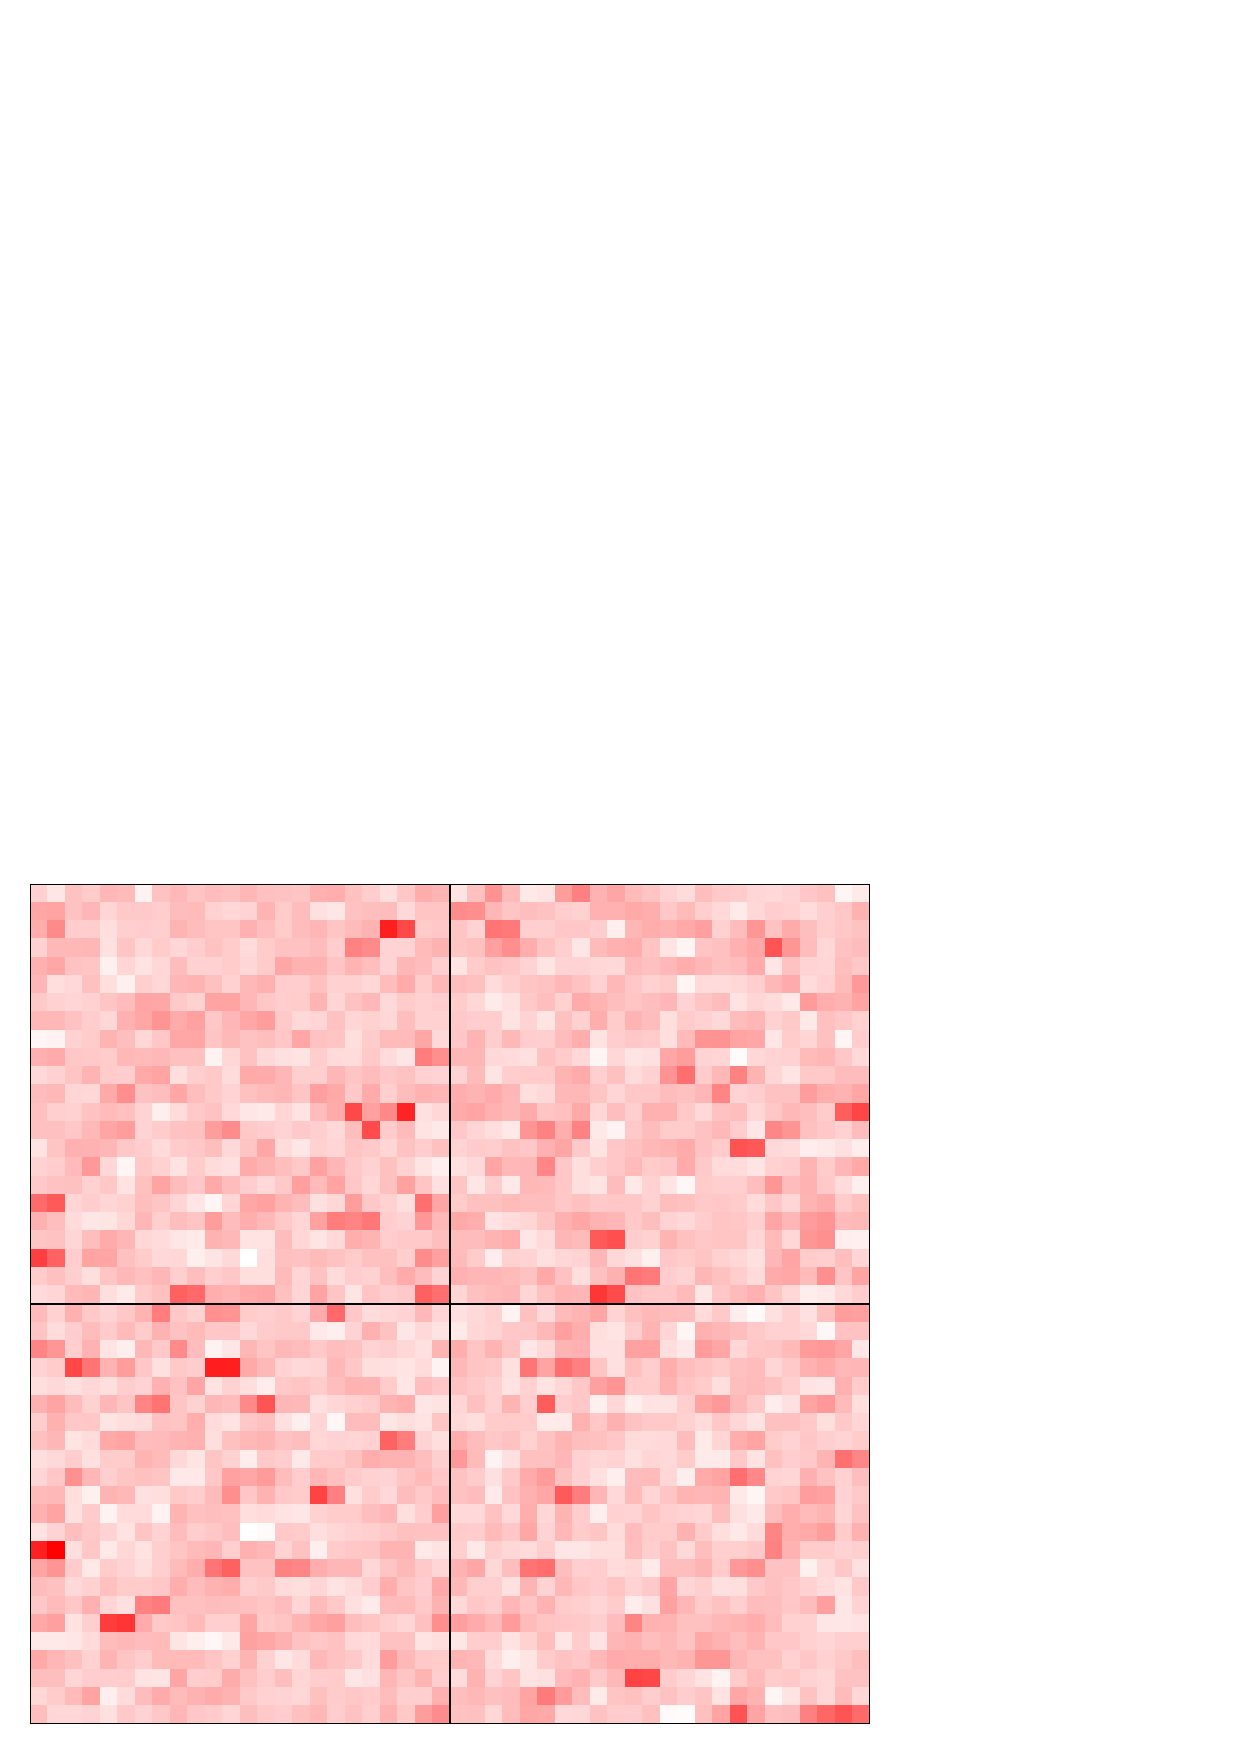
\includegraphics{example-genArise-004}
\caption{Cy3 intensity preview. \label{fig2}}
\end{center}
\end{figure}
\begin{Scode}
> data(Simon)
> datos <- attr(Simon, "spotData")# Extract spot data
> R <- log(datos$Cy3, 2)
> imageLimma(z = R, row = 23, column = 24, meta.row = 2, 
  meta.column = 2, low = "white", high = "red")
\end{Scode}

\begin{Soutput}
Output: Cy3 intensity value
\end{Soutput}
\pagebreak
And this is the plot for Cy5 intensities.
\begin{figure}[h]
\begin{center}
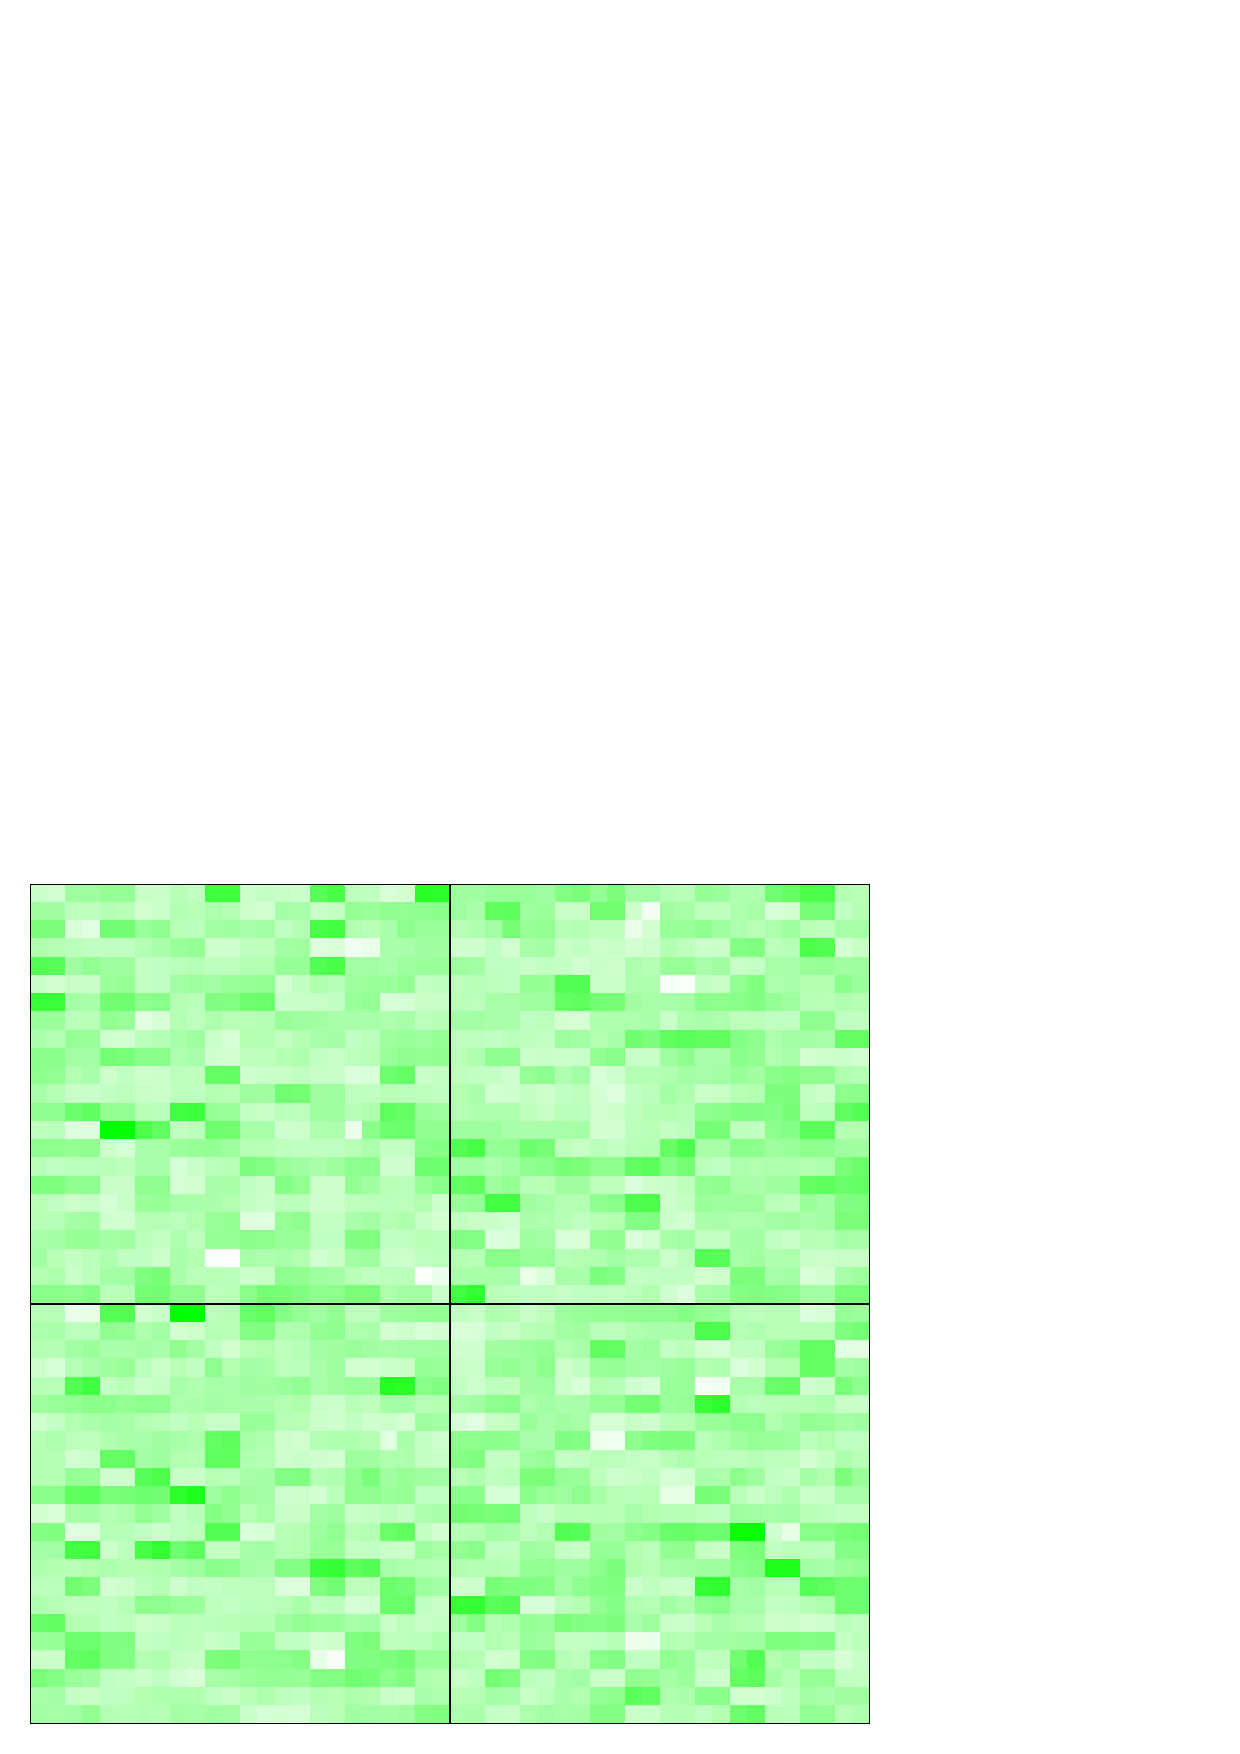
\includegraphics{example-genArise-005}
\caption{Cy5 intensity preview. \label{fig3}}	
\end{center}
\end{figure}
\begin{Scode}
> data(Simon)
> datos <- attr(Simon, "spotData")# Extract spot data
> G <- log(datos$Cy5, 2)
> imageLimma(z = G, row = 23, column = 24, meta.row = 2, 
  meta.column = 2, low = "white", high = "green")
\end{Scode}

\begin{Soutput}
Output: Cy5 intensity value
\end{Soutput}
\pagebreak
The previous plots can show us a preview of the data, but it is important to clarify that this one does not replace the original TIFF image\\

Data analysis requires be able to plot a spot after apply any operation and genArise provides functions for this purpose. For example, we can plot the values R vs I, M vs A and Cy5 vs Cy3. This functions receive an object of the class Spot.
\begin{figure}[h]
\begin{center}
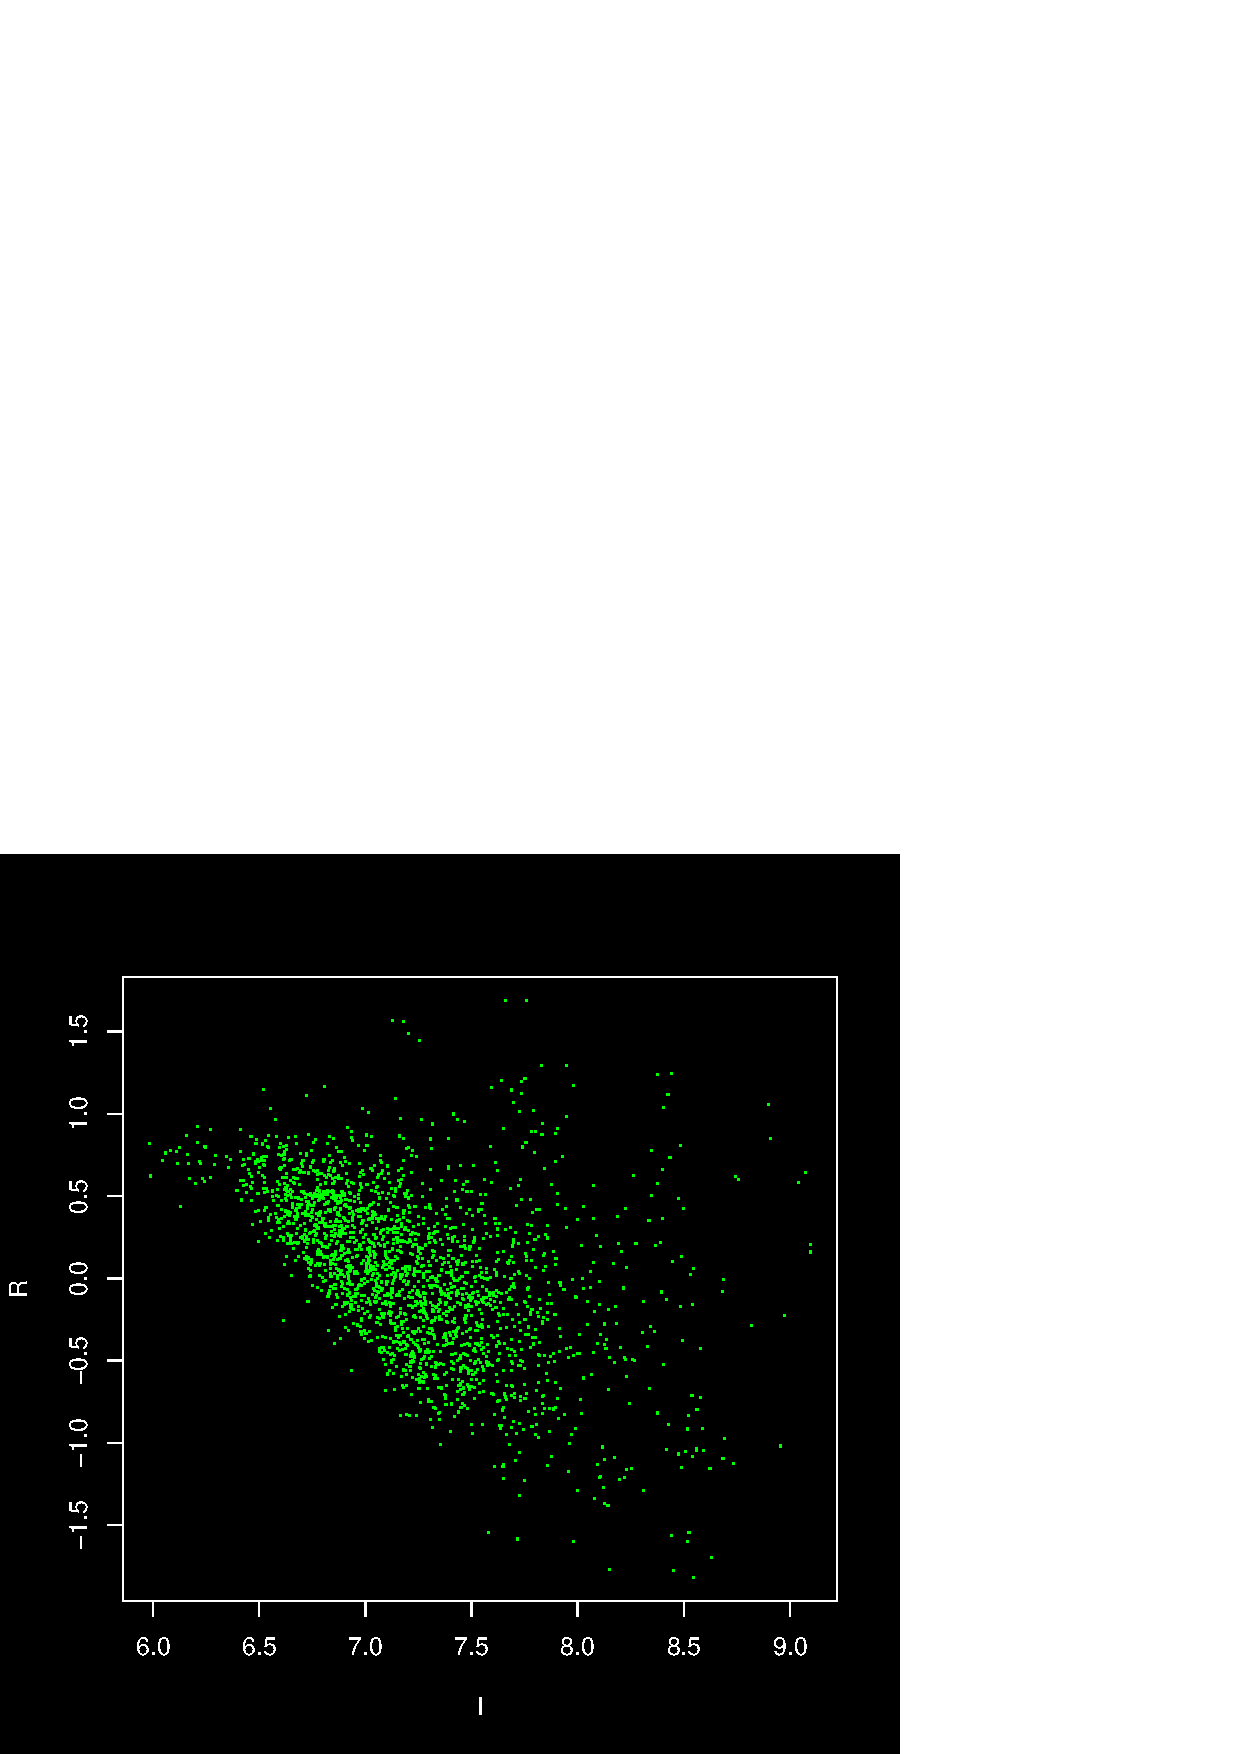
\includegraphics{example-genArise-006}
\caption{R vs I plot. \label{fig4}}	
\end{center}
\end{figure}
\begin{Scode}
> data(Simon)
> ri.plot(Simon)
\end{Scode}
\begin{Soutput}
Output: R vs I plot 
\end{Soutput}
\pagebreak
\begin{figure}[h]
\begin{center}
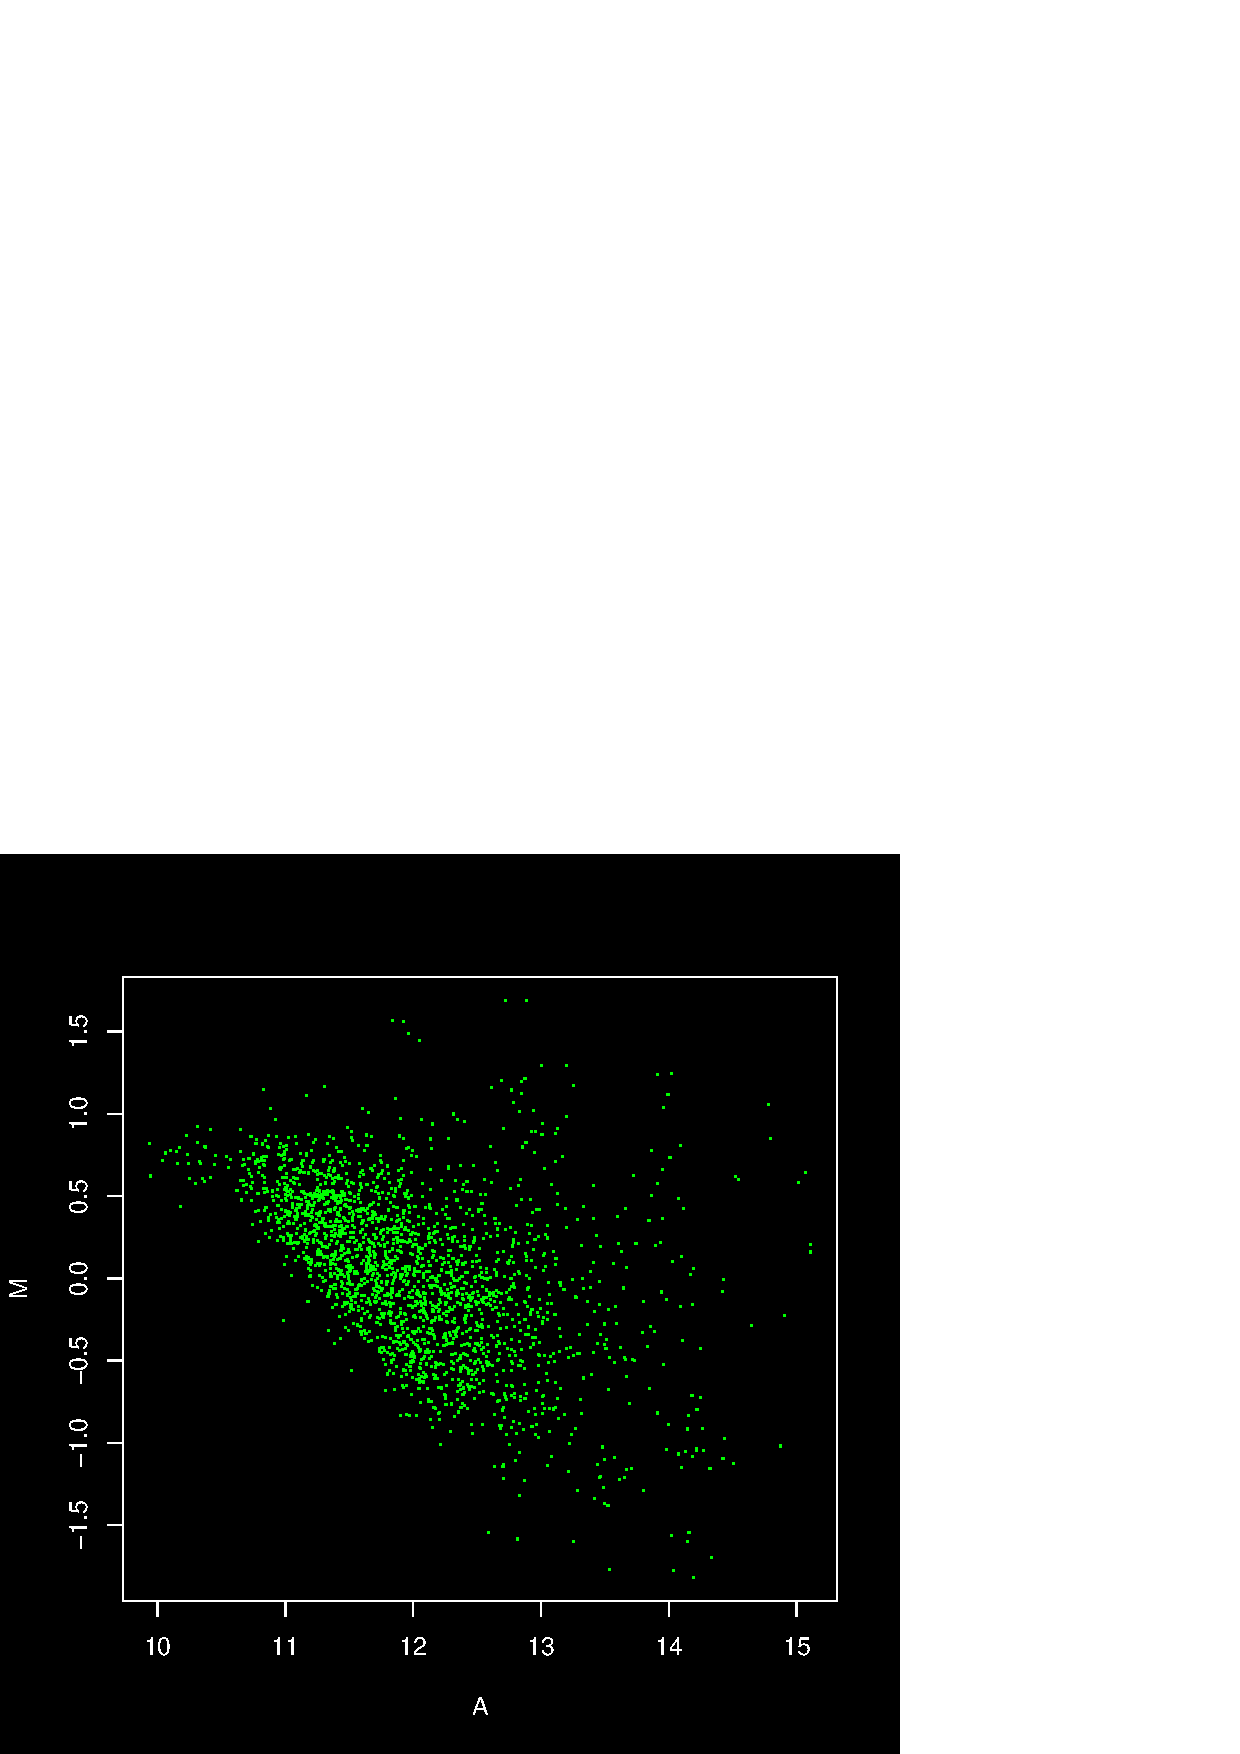
\includegraphics{example-genArise-007}
\caption{M vs A plot. \label{fig5}}
\end{center}
\end{figure}
\begin{Scode}
> data(Simon)
> ma.plot(Simon)
\end{Scode}
\begin{Soutput}
Output: M vs A plot 
\end{Soutput}
\pagebreak
\begin{figure}[h]
\begin{center}
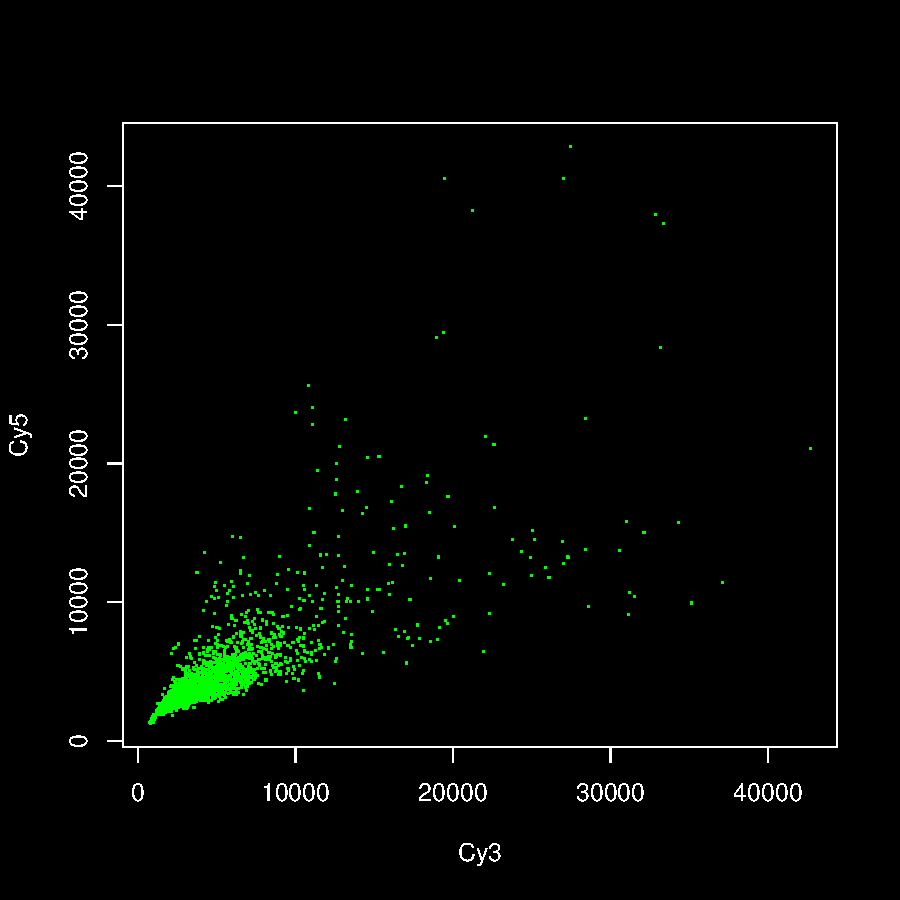
\includegraphics{example-genArise-008}
\caption{Cy3 vs Cy5 plot. \label{fig6}}
\end{center}
\end{figure}
\begin{Scode}
> data(Simon)
> cys.plot(Simon)
\end{Scode}
\begin{Soutput}
Output: plot the Cy3 and Cy5 values
\end{Soutput}
\pagebreak
Once well-known and identified these plots, we can proceed with the data analysis. There are different functions for this purpose. The first of them make the background correction that is a subtraction of backgrounds to the intensity values. The name of this function is \texttt{bg.correct}.
\begin{figure}[h]
\begin{center}
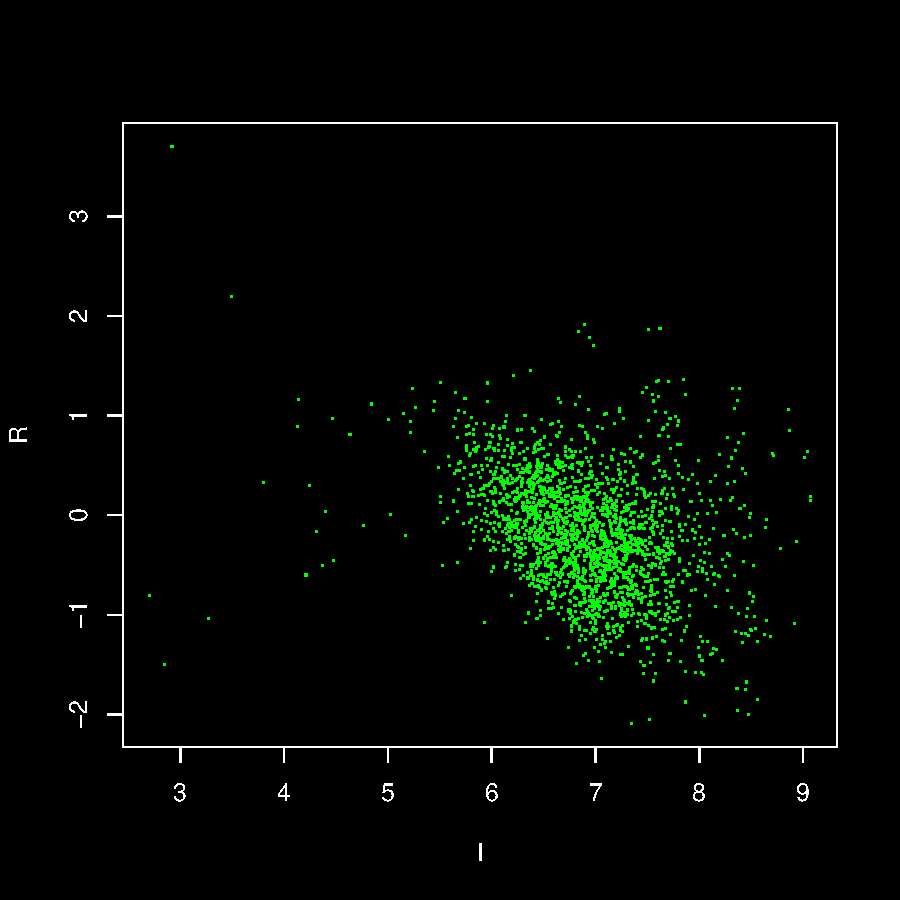
\includegraphics{example-genArise-009}
\caption{Data with background corrected, R vs I. \label{fig7}}
\end{center}
\end{figure}
\begin{Scode}
> data(Simon)
> c.spot <- bg.correct(Simon)
> ri.plot(c.spot)
\end{Scode}

\begin{Soutput}
input: The argument of this function is a spot object
output: A spot objet with the corrected background
\end{Soutput}

The normalization of the data can be done in a global way or by grids, and each one of them returns different results for the same input data set. We must remark that the normalization by grid just can be applied to the complete data set, so we don`t must eliminate observations because we can get some error executing this function.  In the normalization any observation where the R value is zero will be eliminated since it does not have changes in their expression level.\\

The normalization by grid is executed with the function \texttt{grid.norm()} and is mandatory to indicate the dimensions of every grid, so, we must indicate the number of rows and the number of columns that the grid contains.
\begin{figure}[h]
\begin{center}
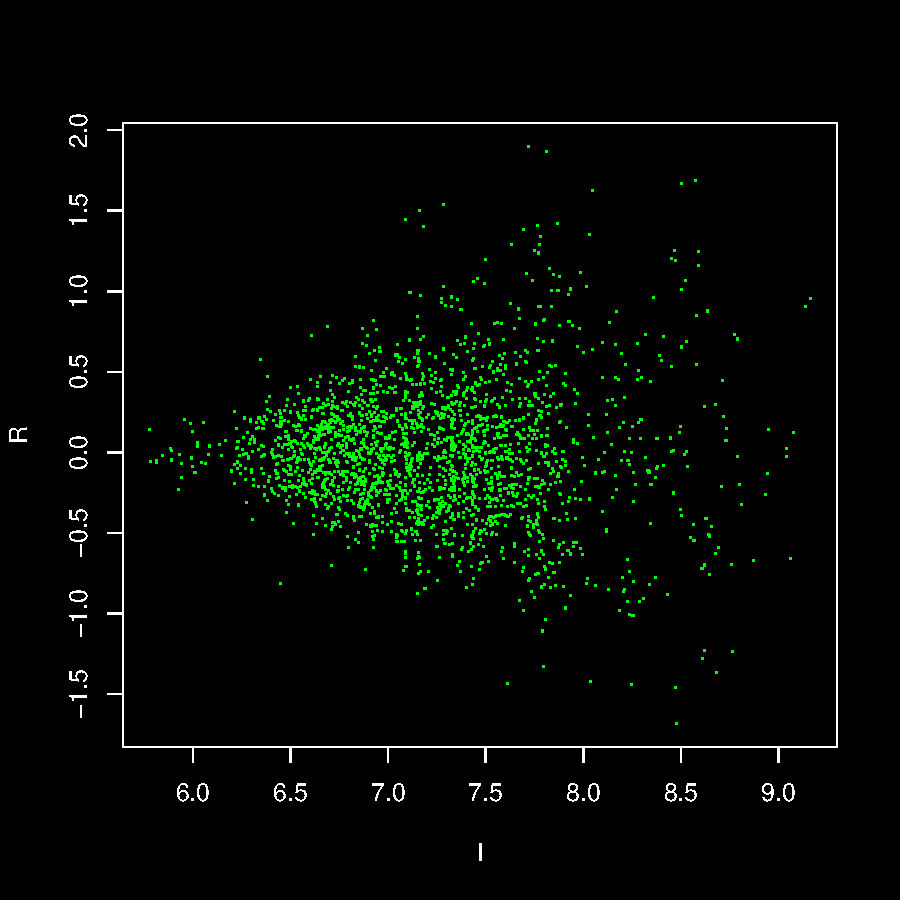
\includegraphics{example-genArise-010}
\caption{Normalized data by grid, R vs I plot \label{fig8}}	
\end{center}
\end{figure}
\begin{Scode}
> data(Simon)
> n.spot <- grid.norm(mySpot = Simon, nr = 23, nc = 24)
> ri.plot(n.spot)
\end{Scode}

\begin{Soutput}
input: The argument of this function is a spot object
       and the grid dimension.
output: A normalized spot objet
\end{Soutput}

\begin{figure}[h]
\begin{center}
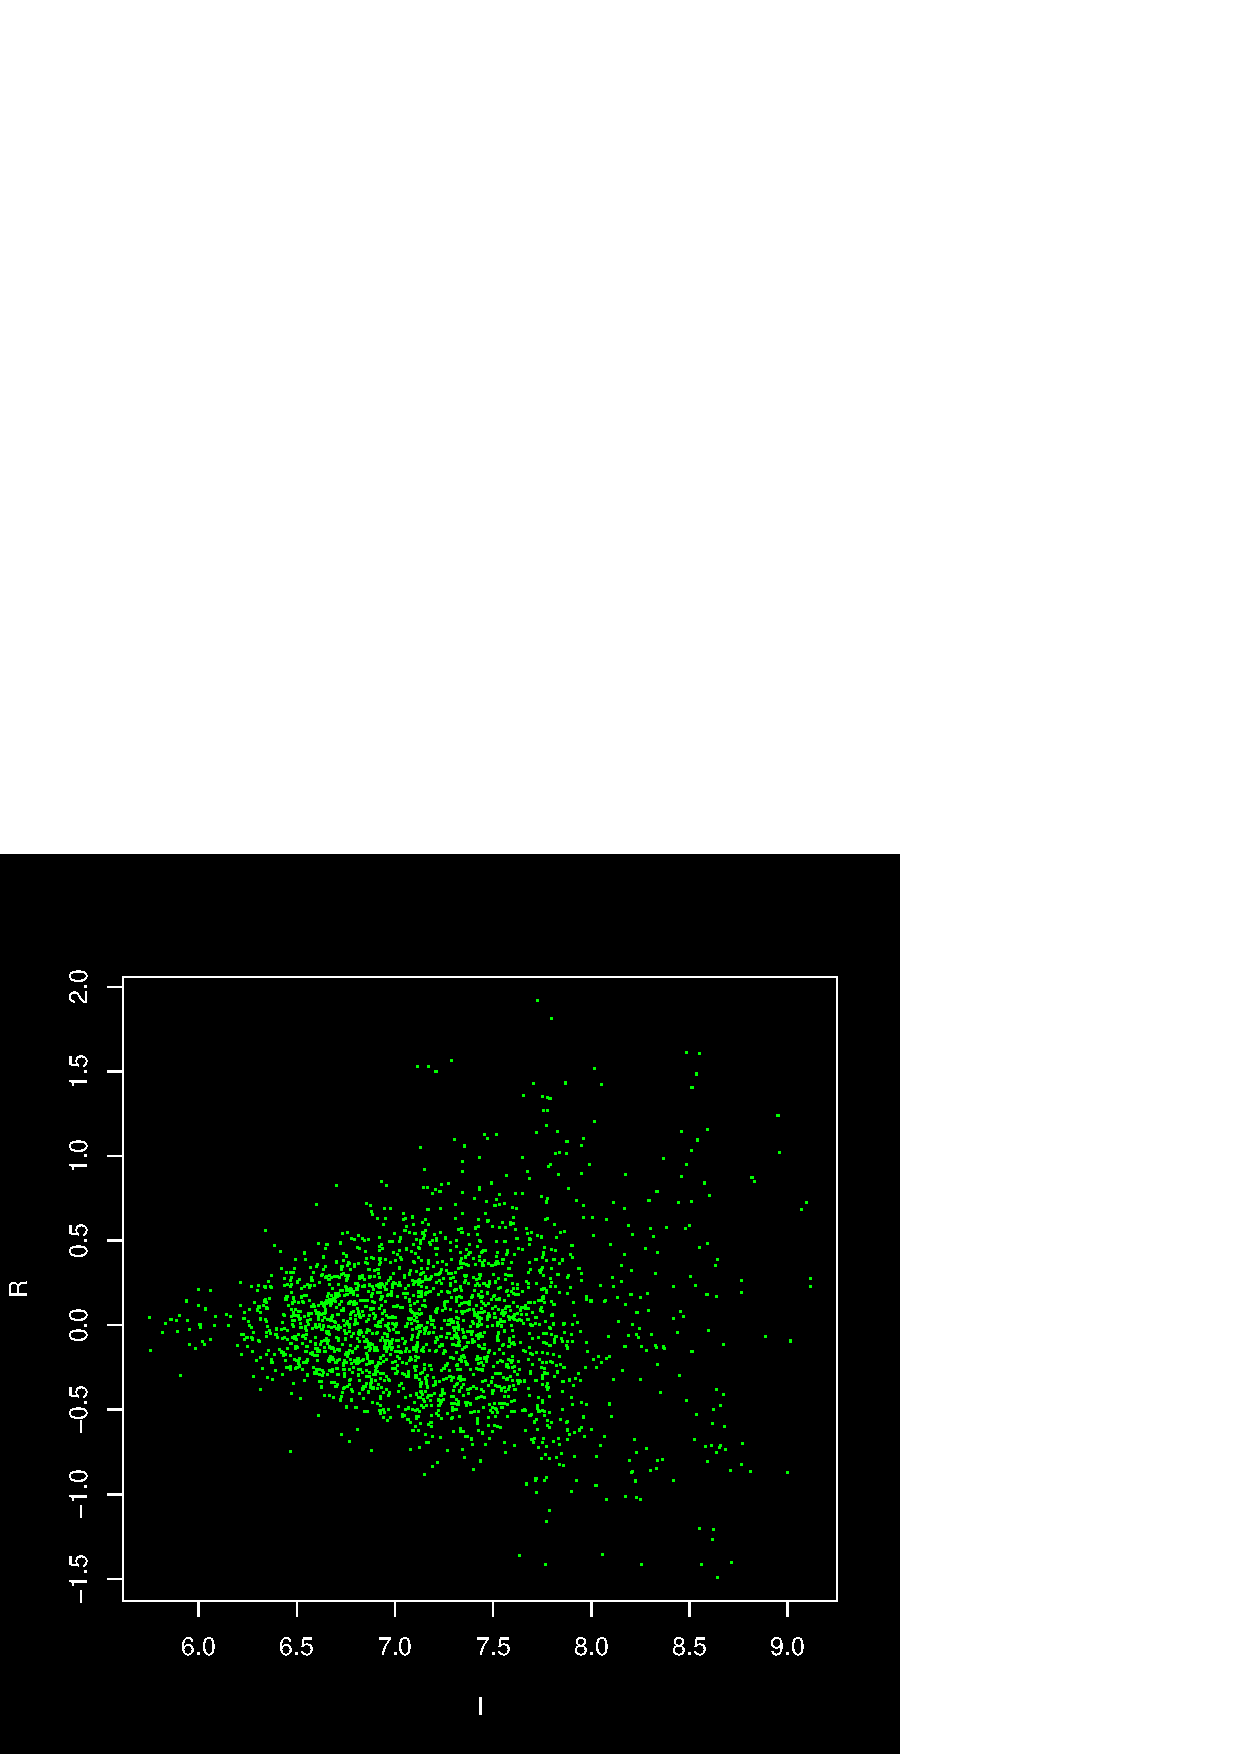
\includegraphics{example-genArise-011}
\caption{Data after global normalisation, R vs I plot. \label{fig9}}
\end{center}
\end{figure}
\begin{Scode}
> data(Simon)
> n.spot <- global.norm(mySpot = Simon)
> ri.plot(n.spot)
\end{Scode}
\begin{Soutput}
Input: The argument of this function is a spot object
Output: A normalized spot objet
\end{Soutput}



On the other hand, the global normalization is executed with the function \texttt{global.norm()} and it only requires as argument an object of the class Spot. As we said previously both functions returns different results and for this reason we must choose the suitable function of normalization to the analysis that we want to do. Remember that once eliminated any observation the normalization by grid can not be done, so in this case this function is the best option.

In this example, the number of data in the spot is small and for this reason the obtained values with both normalization functions could seems very similar in the plots, however this is not the same in all the cases.\\
\pagebreak
The filter of the data is an important step too in the data analysis. genArise implements a filter by low-intensity cutoff. There is a default threshold but you can specify a different one in the moment of the analysis.
\begin{figure}[h]
\begin{center}
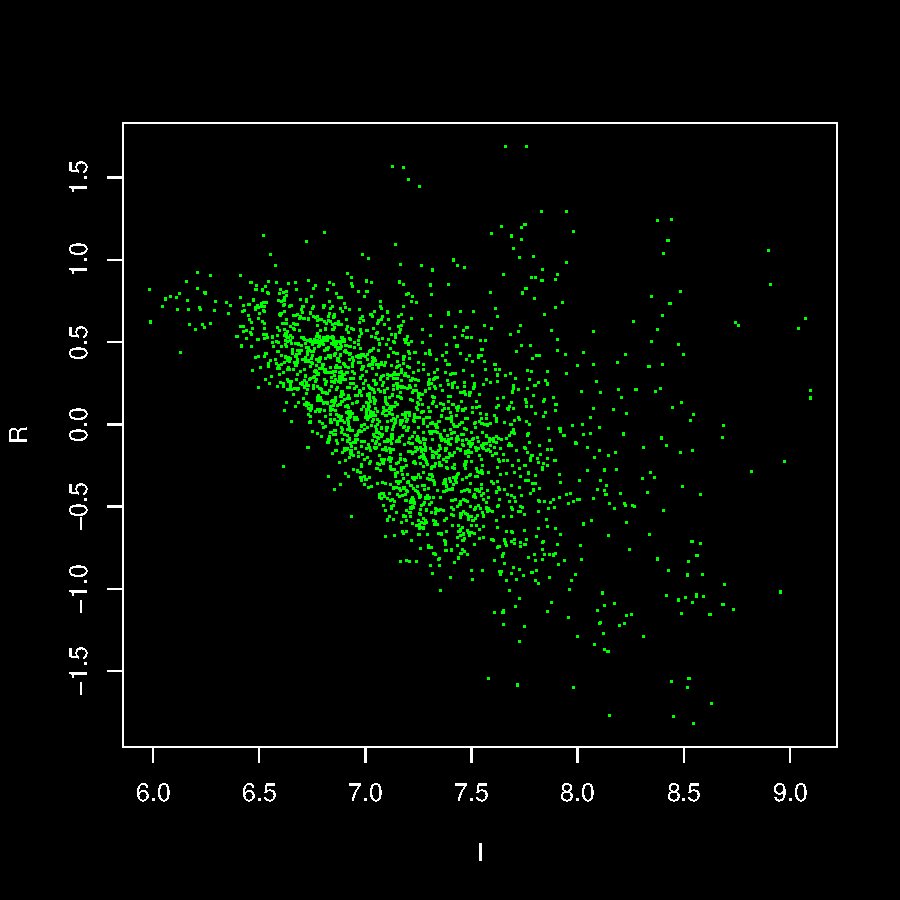
\includegraphics{example-genArise-012}
\caption{Filtered data, R vs I plot \label{fig8}}	
\end{center}
\end{figure}

\begin{Scode}
> data(Simon)
> f.spot <- filter.spot(mySpot = Simon)
> ri.plot(f.spot)
\end{Scode}

\begin{Soutput}
Input: The argument of this function is a spot object.
Output: A filter spot 
\end{Soutput}

Another step is the replicates filtering and in this step a lot of observations are eliminated. We can not just conserve the half of points, but also this function eliminates those points where the diference between the R value of the duplicated observations is bigger than 20\% of one of them. These points are eliminated because it probably means that noise exists and that they are not reliable data to be taken into account in the experiment.
\begin{figure}[h]
\begin{center}
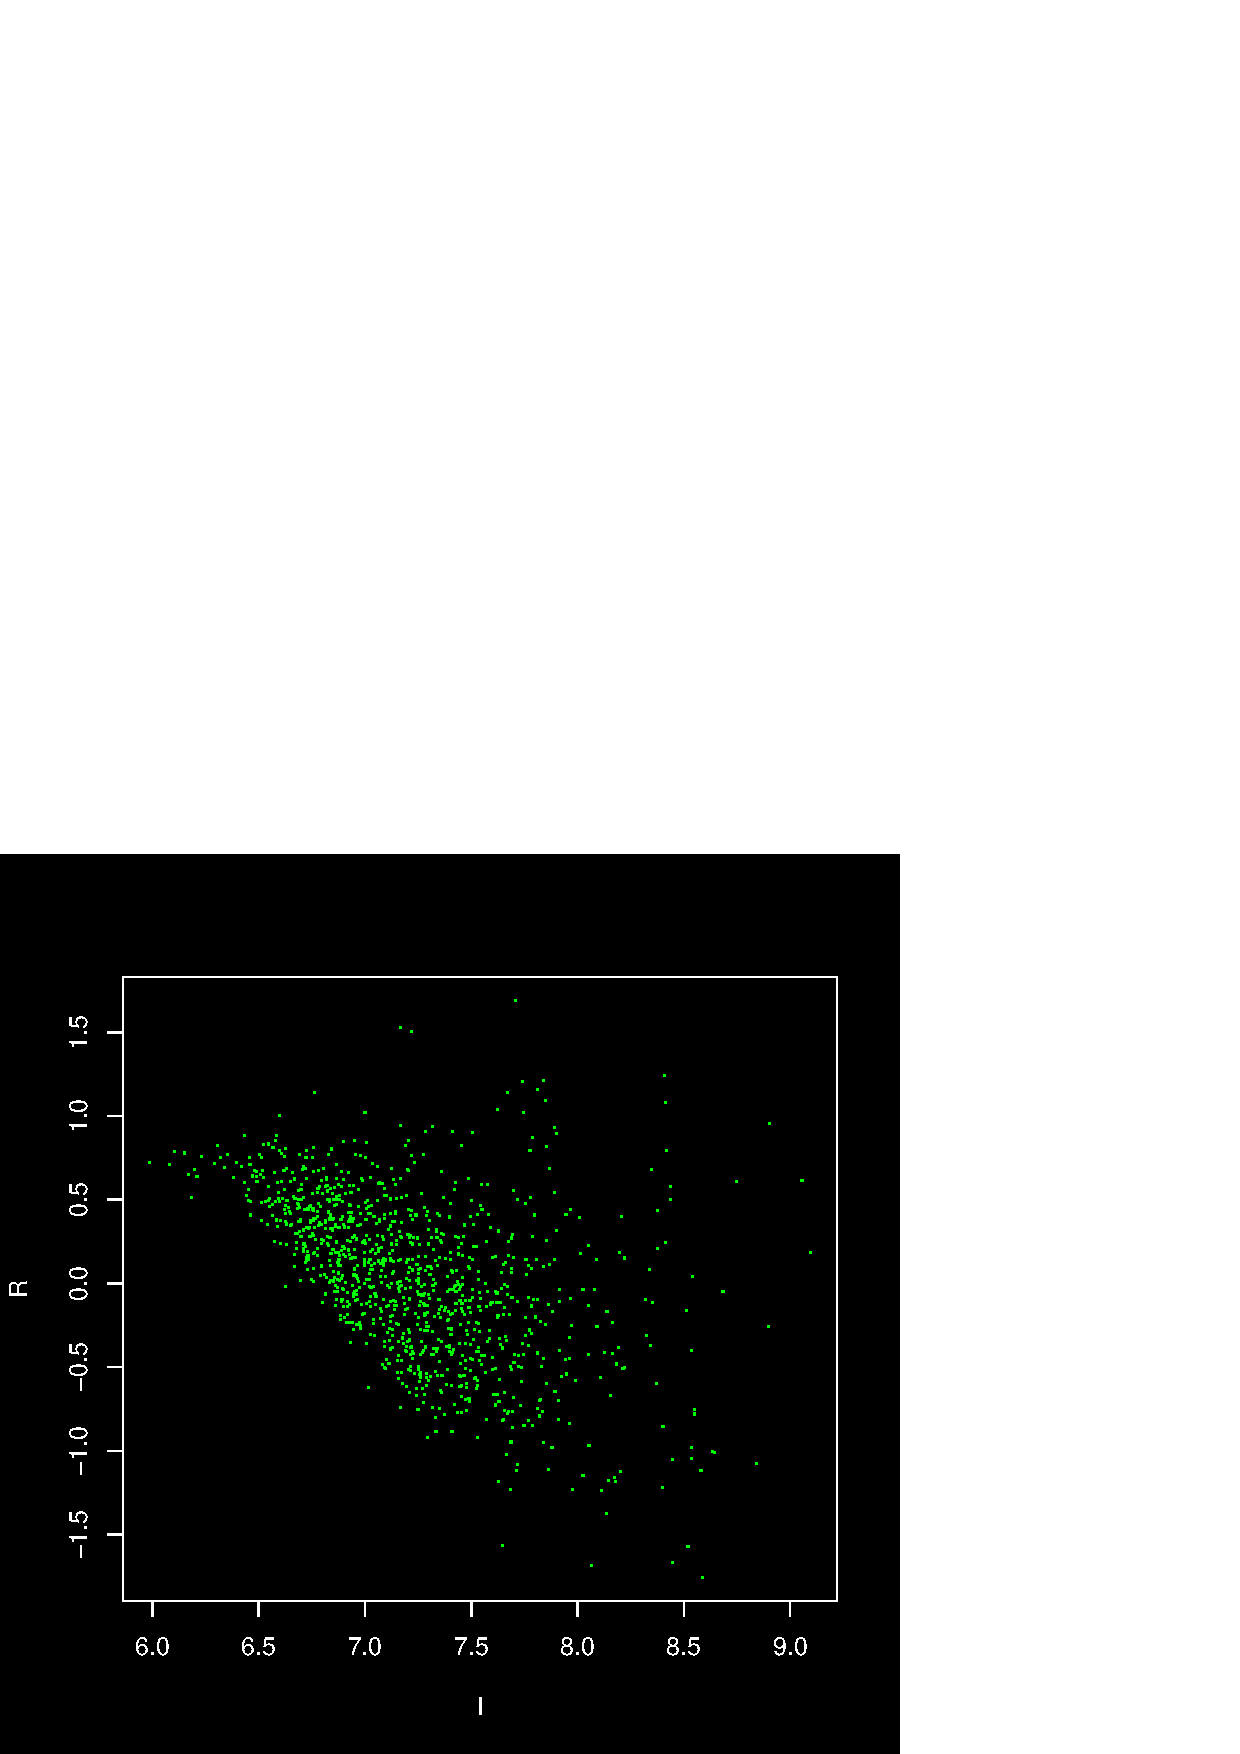
\includegraphics{example-genArise-013}
\caption{Data without duplicates, R vs I\label{fig10}}
\end{center}
\end{figure}
\begin{Scode}
> data(Simon)
> u.spot <- spotUnique(mySpot = Simon)
> ri.plot(u.spot)
\end{Scode}

\begin{Soutput}
Input: The argument of this function is a spot object.
Output: A spot object without duplicates observations
\end{Soutput}

However, genArise offers another functions to the elimination of duplicates different to the previous one. We talk about the function \texttt{alter.unique()}. This function takes the R value of each one of the duplicated observations but just keep that observation with the extremest R value. So, if both of them are positives this function keeps the greater one, if both of them are negatives it keep the lower one and if there is one positive and one negative both observations are eliminated. It is clear that with this function it is conserved a greater number of observations than using the previous algorithm. By this way we probably have at the final of the analysis a greater number of observations in the upper-expressed and lower-expressed because we keep the extreme values.
\begin{figure}[h]
\begin{center}
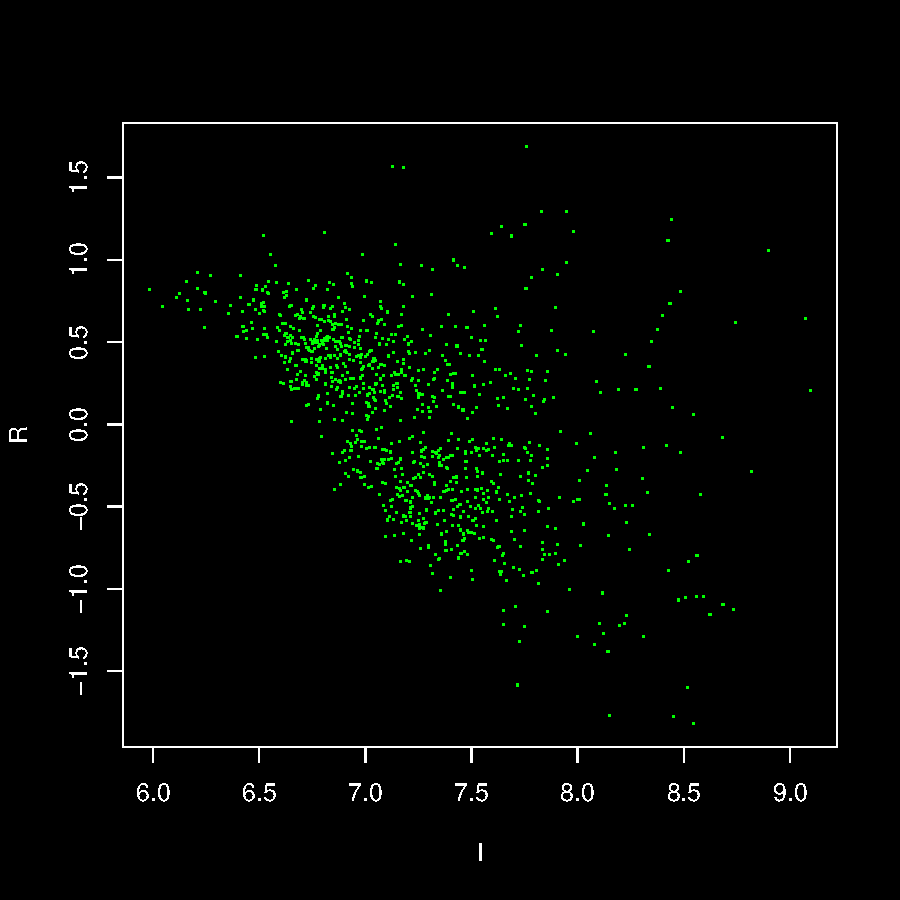
\includegraphics{example-genArise-014}
\caption{Data without duplicated observations.\label{fig11}}
\end{center}
\end{figure}
\begin{Scode}
> data(Simon)
> u.spot <- alter.unique(mySpot = Simon)
> ri.plot(u.spot)
\end{Scode}

\begin{Soutput}
input: The argument of this function is a spot object.
output: A spot object without duplicates observations
\end{Soutput}

The other fuction just get the mean of the duplicates and perform the filtering. The name of this function is \texttt{meanUnique()}.

\begin{figure}[h]
\begin{center}
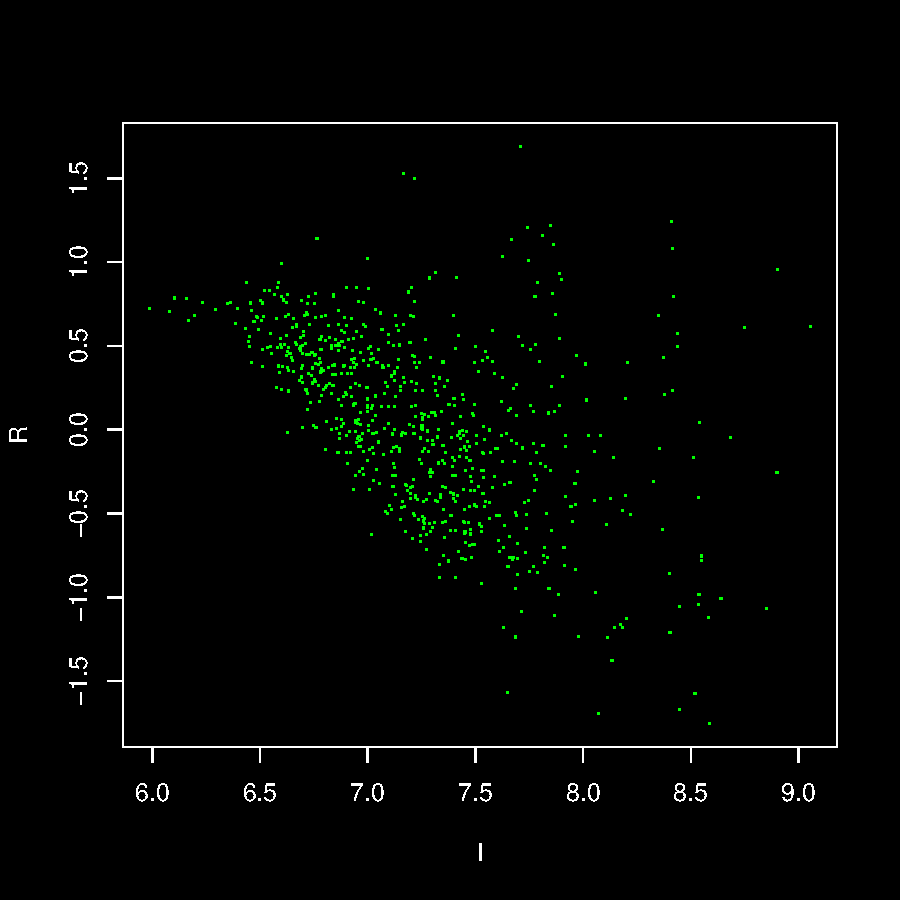
\includegraphics{example-genArise-015}
\caption{Data without duplicated observations.\label{fig11}}
\end{center}
\end{figure}
\begin{Scode}
> data(Simon)
> u.spot <- meanUnique(mySpot = Simon)
> ri.plot(u.spot)
\end{Scode}

\begin{Soutput}
input: The argument of this function is a spot object
output: A spot object without duplicates observations
\end{Soutput}

The intensity-dependent Z-score function allows identify and classify array elements depending on the standard deviations they are from the mean.\\

As a matter of fact genArise offers two options for this analysis. You just need to specify in the type argument on the Zscore function if you want a R-I or a M-A analysis.The first one slide the window along the I value axis and the second slide the window along the A value axis. This function receive as argument an object of the class Spot and returns an object of another class called DataSet that has a different format.\\

This is the example for \texttt{Zscore}

\begin{Scode}
> data(Simon)
> s.spot <- Zscore(Simon, type="ri")
\end{Scode}

\begin{Soutput}
Input: The argument of this function is a spot object
Output: An object of the class DataSet
\end{Soutput}

And this is the example for \texttt{M-A} analysis

\begin{Scode}
> data(Simon)
> s.spot <- Zscore(Simon, type="ma")
\end{Scode}

\begin{Soutput}
Input: The argument of this function is a spot object
Output: An object of the class DataSet
\end{Soutput}

Since the objects of the class DataSet are different to the objects of the class Spot we need a function to plot them. For this purpose exists a function called \texttt{Zscore.plot}.So, in a R-I plot, array elements are color-coded depending on wether they are less than 1 standard deviation from the mean (blue), between 1 and 1.5 standard deviations (green), between 1.5 and 2 sd (red), or more than 2 standard deviations from the mean (orange).
\begin{figure}[h]
\begin{center}
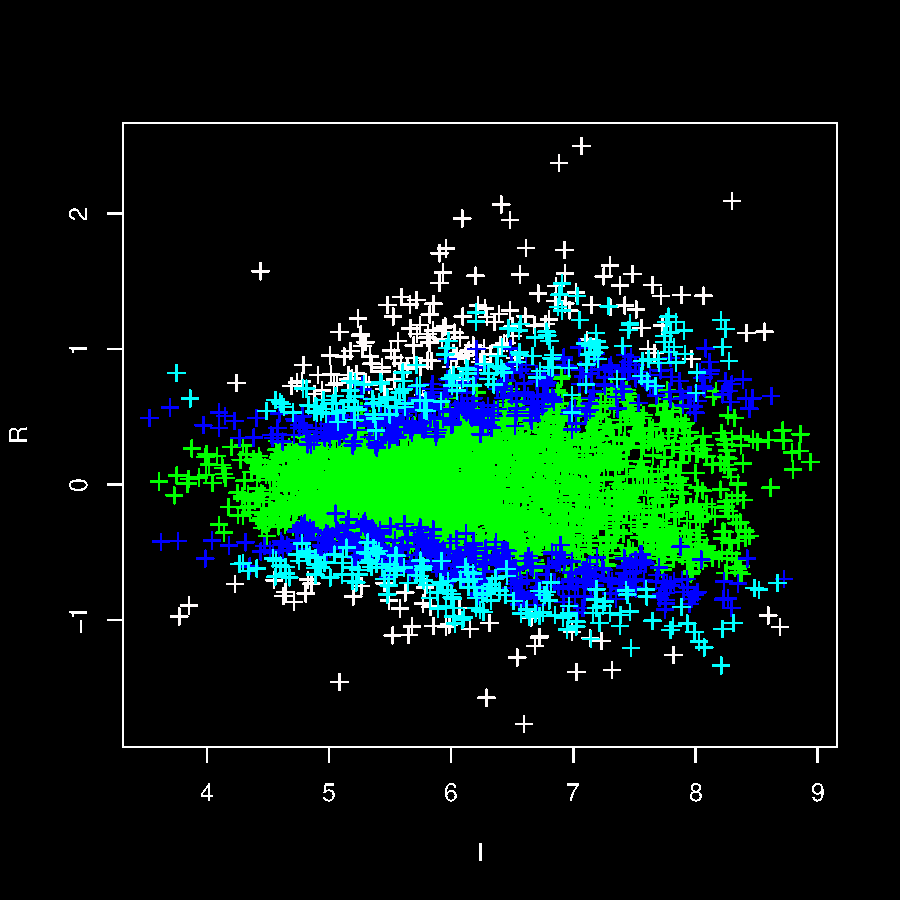
\includegraphics{example-genArise-016}
\caption{Data after Z-score Analysis. \label{fig12}}
\end{center}
\end{figure}
\begin{Scode}
> data(WT.dataset)
> Zscore.plot(WT.dataset)
\end{Scode}

\begin{Soutput}
Input: A object of the class DataSet
Output: Plot for identify differential expression
\end{Soutput}

With the upper-expressed and lower-expressed sets, or together or separated we can start a post-analysis with a function called genMerge. This function allows analyze the functional genomic data related with the genes located in upper and lower sets.

Given a set of genes (for example the upper-expressed), genMerge writes in a files the data of an statistic analysis of the upper/representation of functions or particular categories on the set of data upper-expressed.\\

We must take care in the format of the input file. No one parameter file should have header. This function requires four data files and the file name where will be save the obtained information. The main file that the function needs are:\\
\textbf{Association file}. This file contains two columns separated by tabs. The first column corresponds to the gen identifier in the microarray and the second one corresponds to a list of associated GOs to this gen. Each GO in this list is separted by ";" and is necesary to consult a database to locate the associated GOs to each gen (see htttp://genontology.org)
\begin{Scode}
Example:

YAL001C GO:0003709;
YAL002W GO:0005554;
YAL003W GO:0003746;
YAL005C GO:0003754;GO:0003773;GO:0004002;
YAL007C GO:0005554;
\end{Scode}

\textbf{Description file}. This file also contains two columns separated by tabs, the first corresponds to the name of some GOs and the second corresponds to the description associated to each GO in the database.
\begin{Scode}
Example:

GO:0000005      ribosomal chaperone activity
GO:0000006      high affinity zinc uptake transporter activity
GO:0000007      low-affinity zinc ion transporter activity
GO:0000008      thioredoxin
GO:0000009      alpha-1,6-mannosyltransferase activity
GO:0000010      trans-hexaprenyltranstransferase activity
GO:0000014      single-stranded DNA specific endodeoxyribonuclease activity
GO:0000016      lactase activity
\end{Scode}

\textbf{All genes (population.genes)}. This file only should contains one column, the spot identifiers or those of the input file not analyzed yet are the column information, each identifier is a row file. 
\begin{Scode}
YAL001C
YAL002W
YAL003W
YAL004W
YAL005C
YAL007C
YAL008W
YAL009W
YAL010C
YAL011W
\end{Scode}

\textbf{The genes to study}. Like the preceding described file, this file only contains one column and each row correspond to the name of one of the genes in the set that will be studied (upper-expressed or lower-expressed). The function sintax is the next one:

\begin{Scode}
> # Let's suppose that original spot is o.spot
> # To write the population file you can use write.table
> ids <- atrr(o.spot, "spotData")$Ids
> ids <- unique(ids)
> write.table(ids, "population.genes")
\end{Scode}

\begin{Soutput}
Input: An object of class Slice
Output: Plot upper-expressed and lower-expressed
\end{Soutput}

In the same way, we write the identifiers of the genes set that will be studied. Suppose there exist a slice Spot we call s.spot wich have the results after slice analysis, if we wish that our set of study have the upper-expressed identifiers and the lower-expressed identifiers to write the corresponding file we must follow the next code.

\begin{Scode}
> # To write the study genes file
> study.ids <- c(s.spot$Id.up, s.spot$Id.down)
> study.ids <- unique(study.ids) 
> write.table(study.ids, "study.genes")
\end{Scode}

If we only want to preserve the identifier of some set, say upper-expressed or lower-expressed type the next lines:

\begin{Scode}
> # Only write upper-expressed
> study.ids <- s.spot$Id.up # to write lower-expressed use s.spot$Id.down
> study.ids <- unique(study.ids)
> write.table(study.ids, "study.genes")
\end{Scode}

The other files should be constructed consulting a database or could be downloaded from internet, this files should contain the format described above, so that the genMerge function operates correctly. The sintax of this is:   

\begin{Scode}
> genMerge(gene.association, description, population.genes, study.genes, output.file = "GenMerge.txt"){
\end{Scode}

The results will be in the corresponding file.

\section{The genArise GUI}

For make easier the analysis, genArise joins all functions in a single one with a graphic interface, to call this function we type the next line:

\begin{Scode}
> genArise()
\end{Scode}

Now the next menu is displayed.
\begin{figure}[h]
\begin{center}

\includegraphics[scale= 0.3]{./images/mainmenu.pdf}\\
\caption{genArise Menu. \label{fig1}}
\end{center}
\end{figure}

Once in this menu we should create a New Project following the sequence  \textbf{File $\rightarrow$ Project $\rightarrow$ New Project}.\\
The last step displays a window where we should indicate the file' s location containing the data to analyze, indicating whether the file is a foreing experiment or belong to one made in the Cellular Physiology Institute UNAM. 
\begin{figure}[h]
\begin{center}
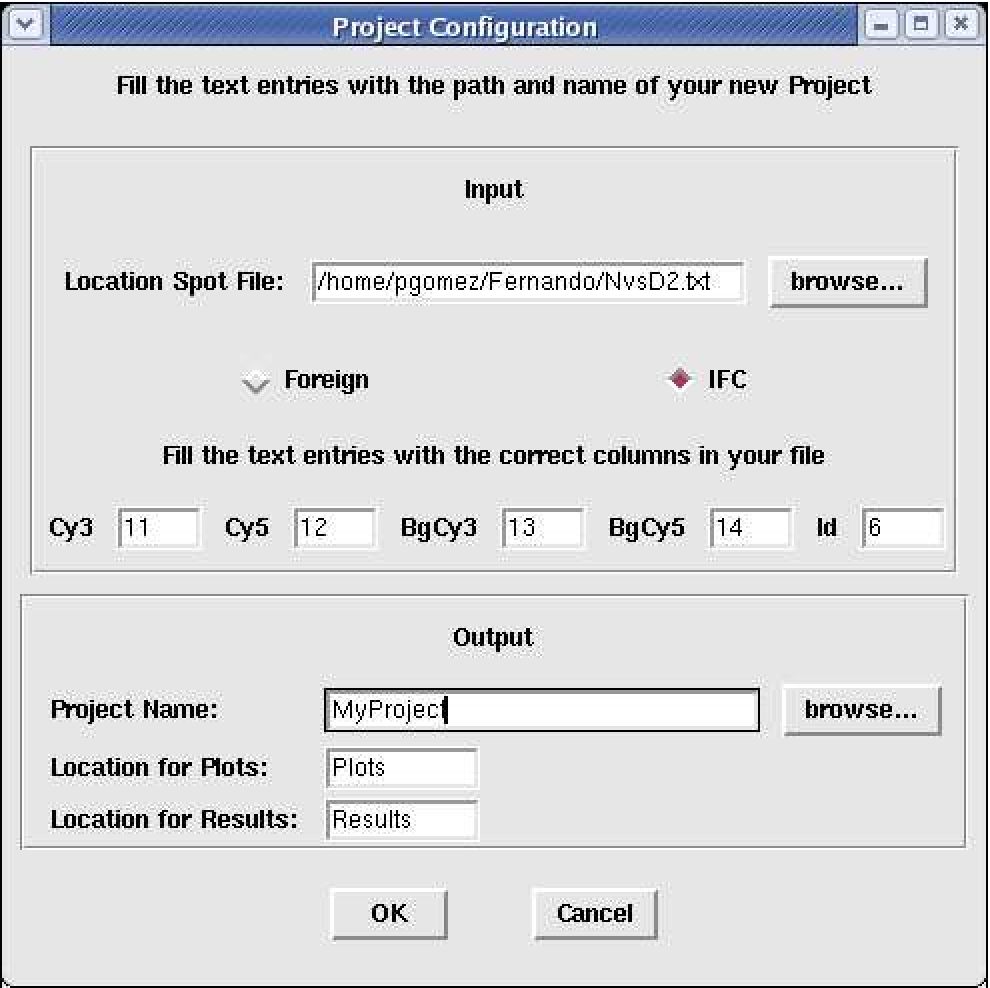
\includegraphics[scale= 0.3]{./images/projectmenufilled.pdf}\\
\caption{Project Configuration Window. \label{fig2}}
\end{center}
\end{figure}

In the lower textfields we should indicate the location and name of the new project containing the results and graphics obtained during the analysis.\\
 For example:\\
 \\
The image above shows an analysis that will be made on the file Rat\_5k\_014.csv containig a microarray made in the Cellular Physiology Institute' s Microarray Unit. We call the project ProjectRat. The default name for the graphics directory is Plot and for the data files is Results. If we wish modify this names we just change the names that appear in the options \textbf{Location for Plots } and \textbf{Location for Results } respectively.\\

Then, the window containing a preliminary view of the spot is displayed to verify that there  exist any error in the experiment. It's important make clear that these images don't substitute the TIFF file.

\begin{figure}[h]
\begin{center}
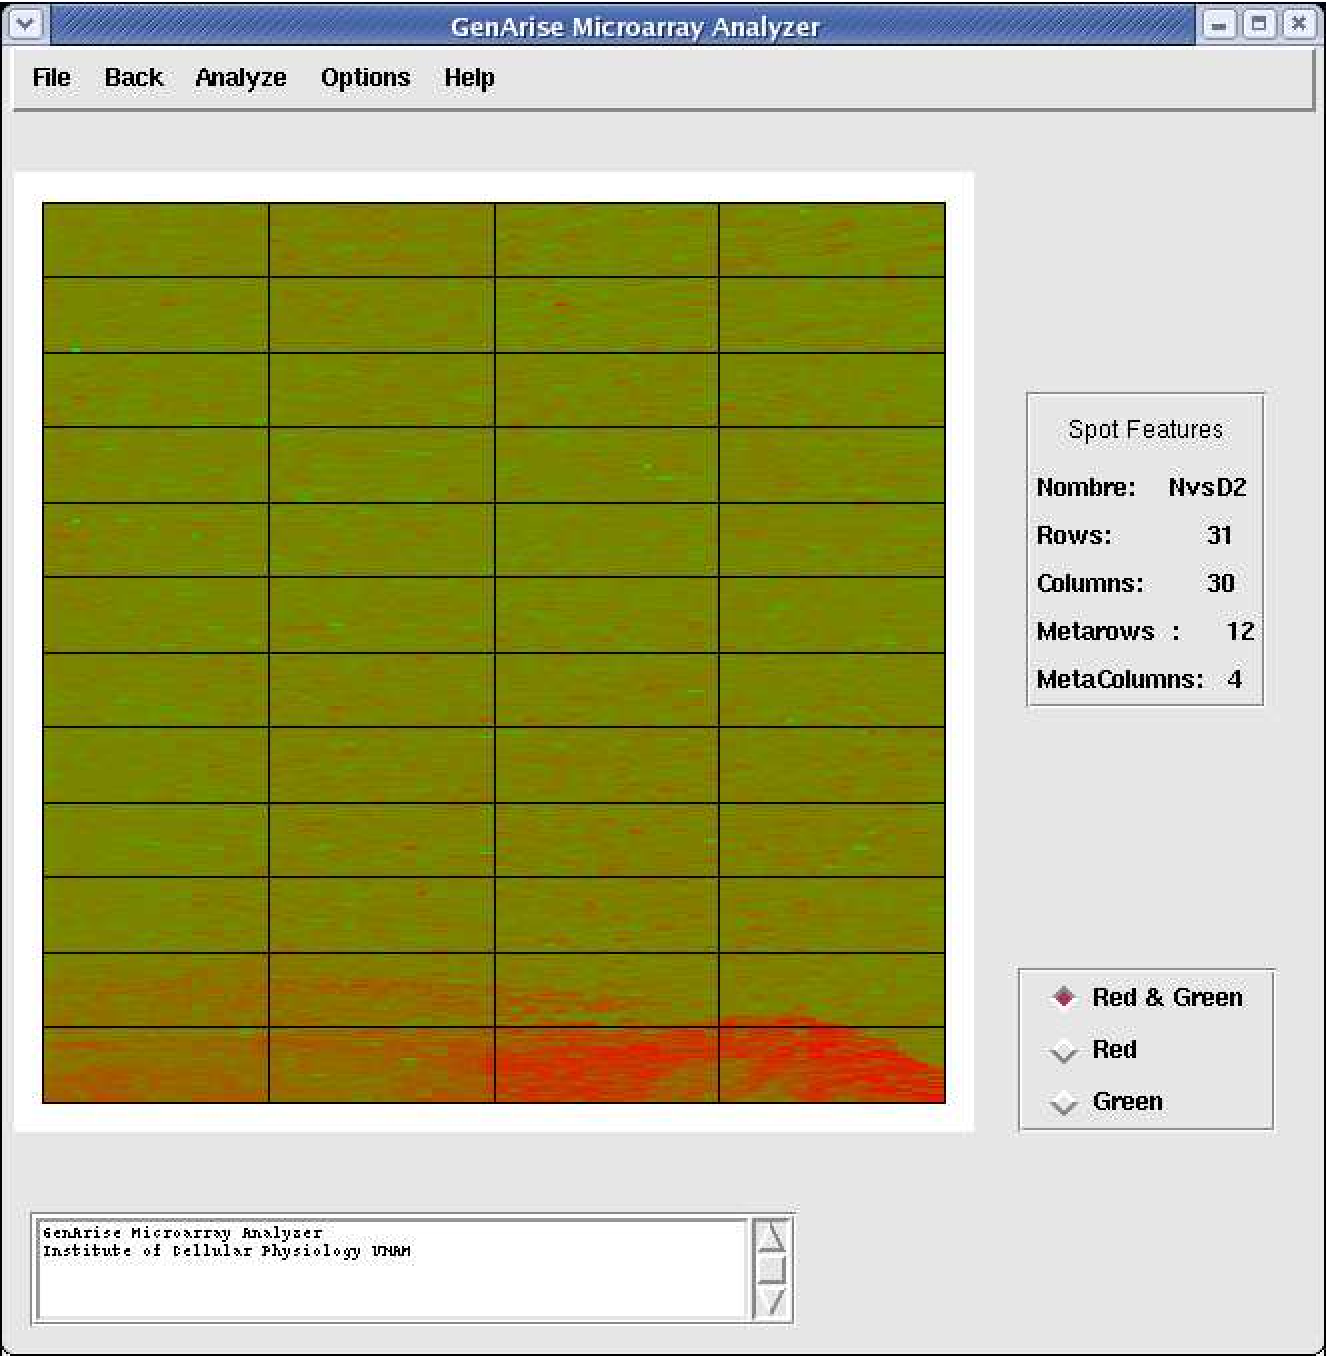
\includegraphics[scale= 0.3]{./images/principal.pdf}\\
\caption{Preview Window, plotting Cy3 and Cy5 intensities mixed\label{fig3}}
\end{center}
\end{figure}
We also can see the green and red levels in a separated form just by pressing the radiobuttons in the lower right part of the window.
\begin{figure}[h]
\begin{center}
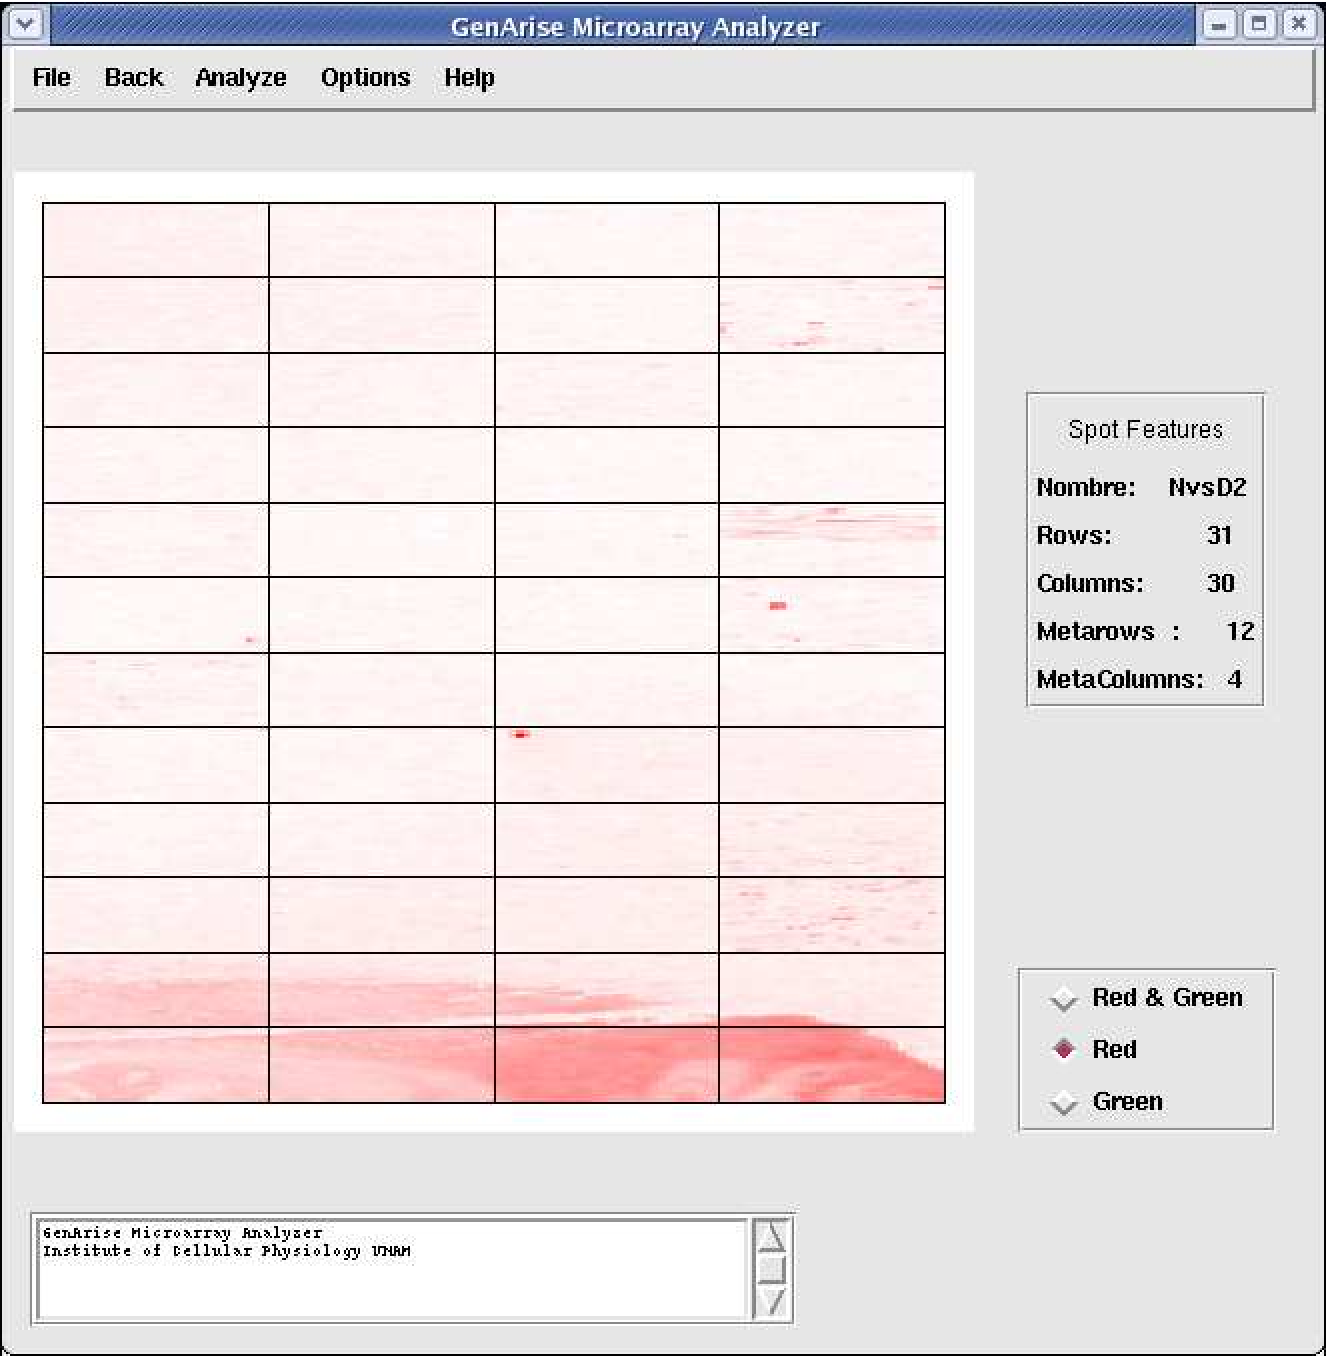
\includegraphics[height=3.in,width=3.15in]{./images/principalRed.pdf}\\
\caption{Preview Window, plotting Cy3 intensity value. \label{fig4}}
\end{center}
\end{figure}
\textbf{\\\\}
\begin{figure}[h]
\begin{center}
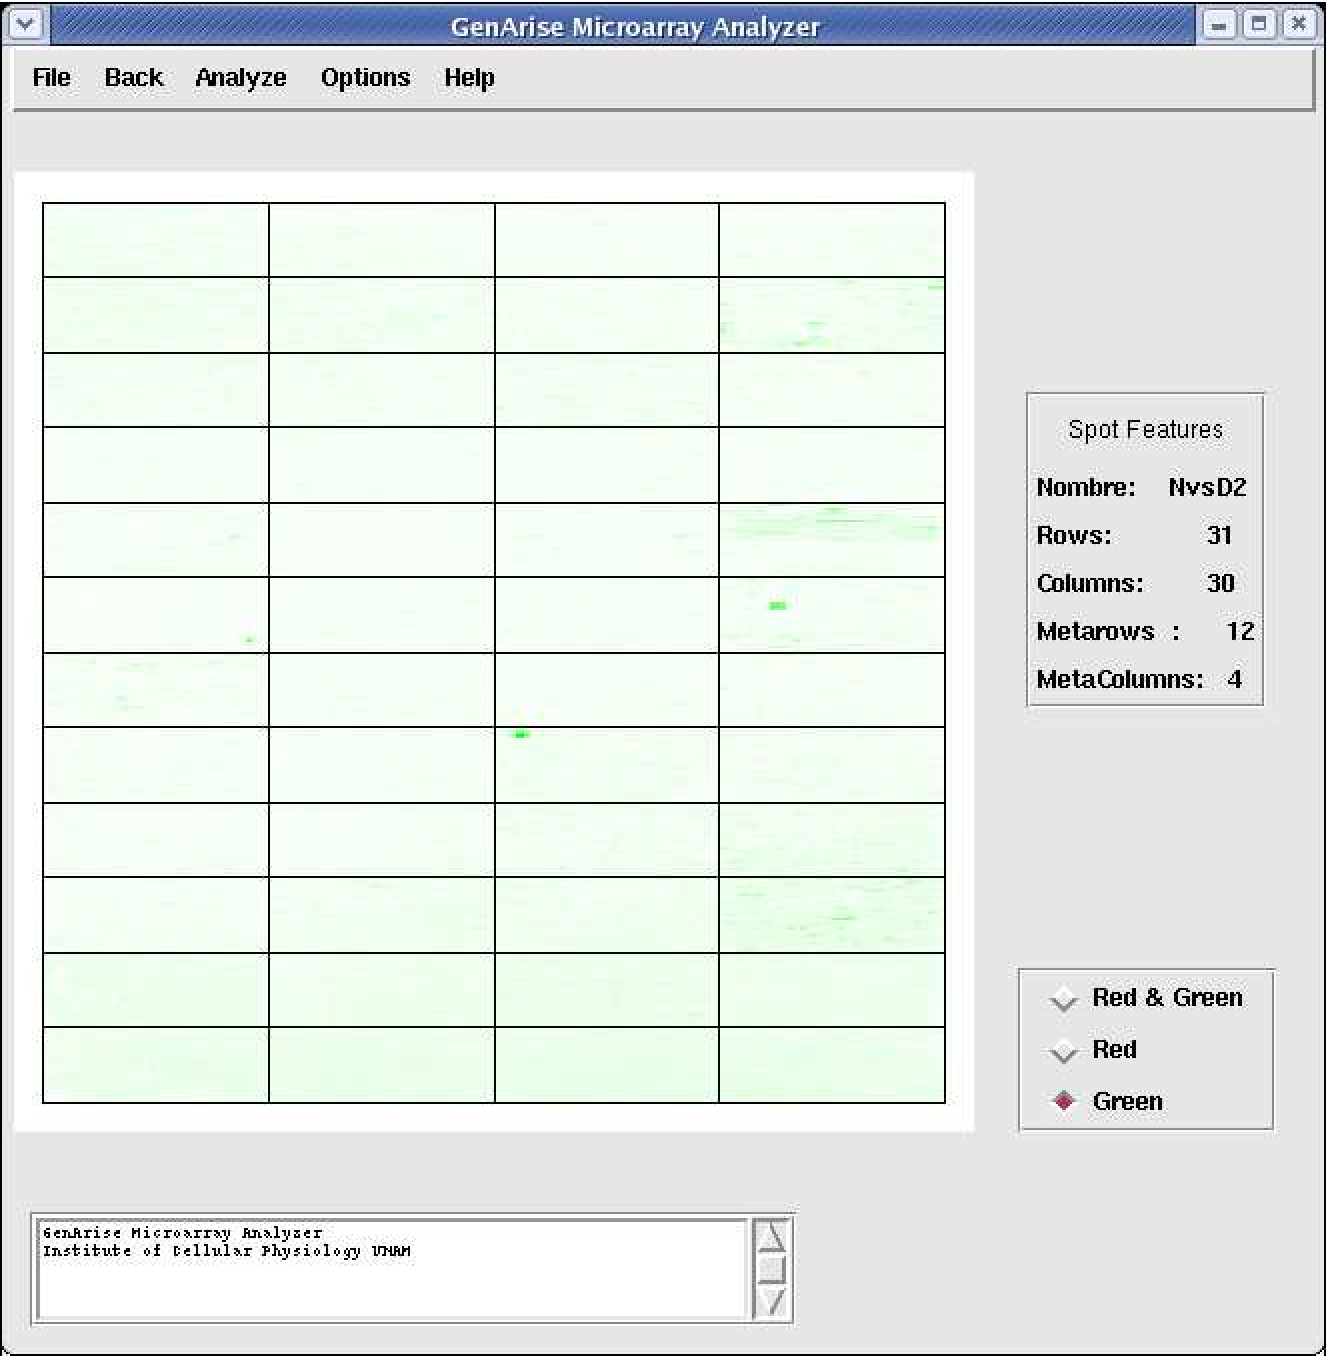
\includegraphics[height=3in,width=3.15in]{./images/principalGreen.pdf}\\
\caption{Preview Window, plotting Cy5 intensity value. \label{fig5}}
\end{center}
\end{figure}

In the upper right side of the window we can see the data attributes of the file that is being analyzed and the experiment configuration.\\
We can save the plot in a pdf file by selecting the option \textbf{Save as PDF} in the menu Options. With the option Annotations of the same menu we can make some important annotations through the analysis and save these in a file called annotations.txt.
\begin{figure}[h]
\begin{center}
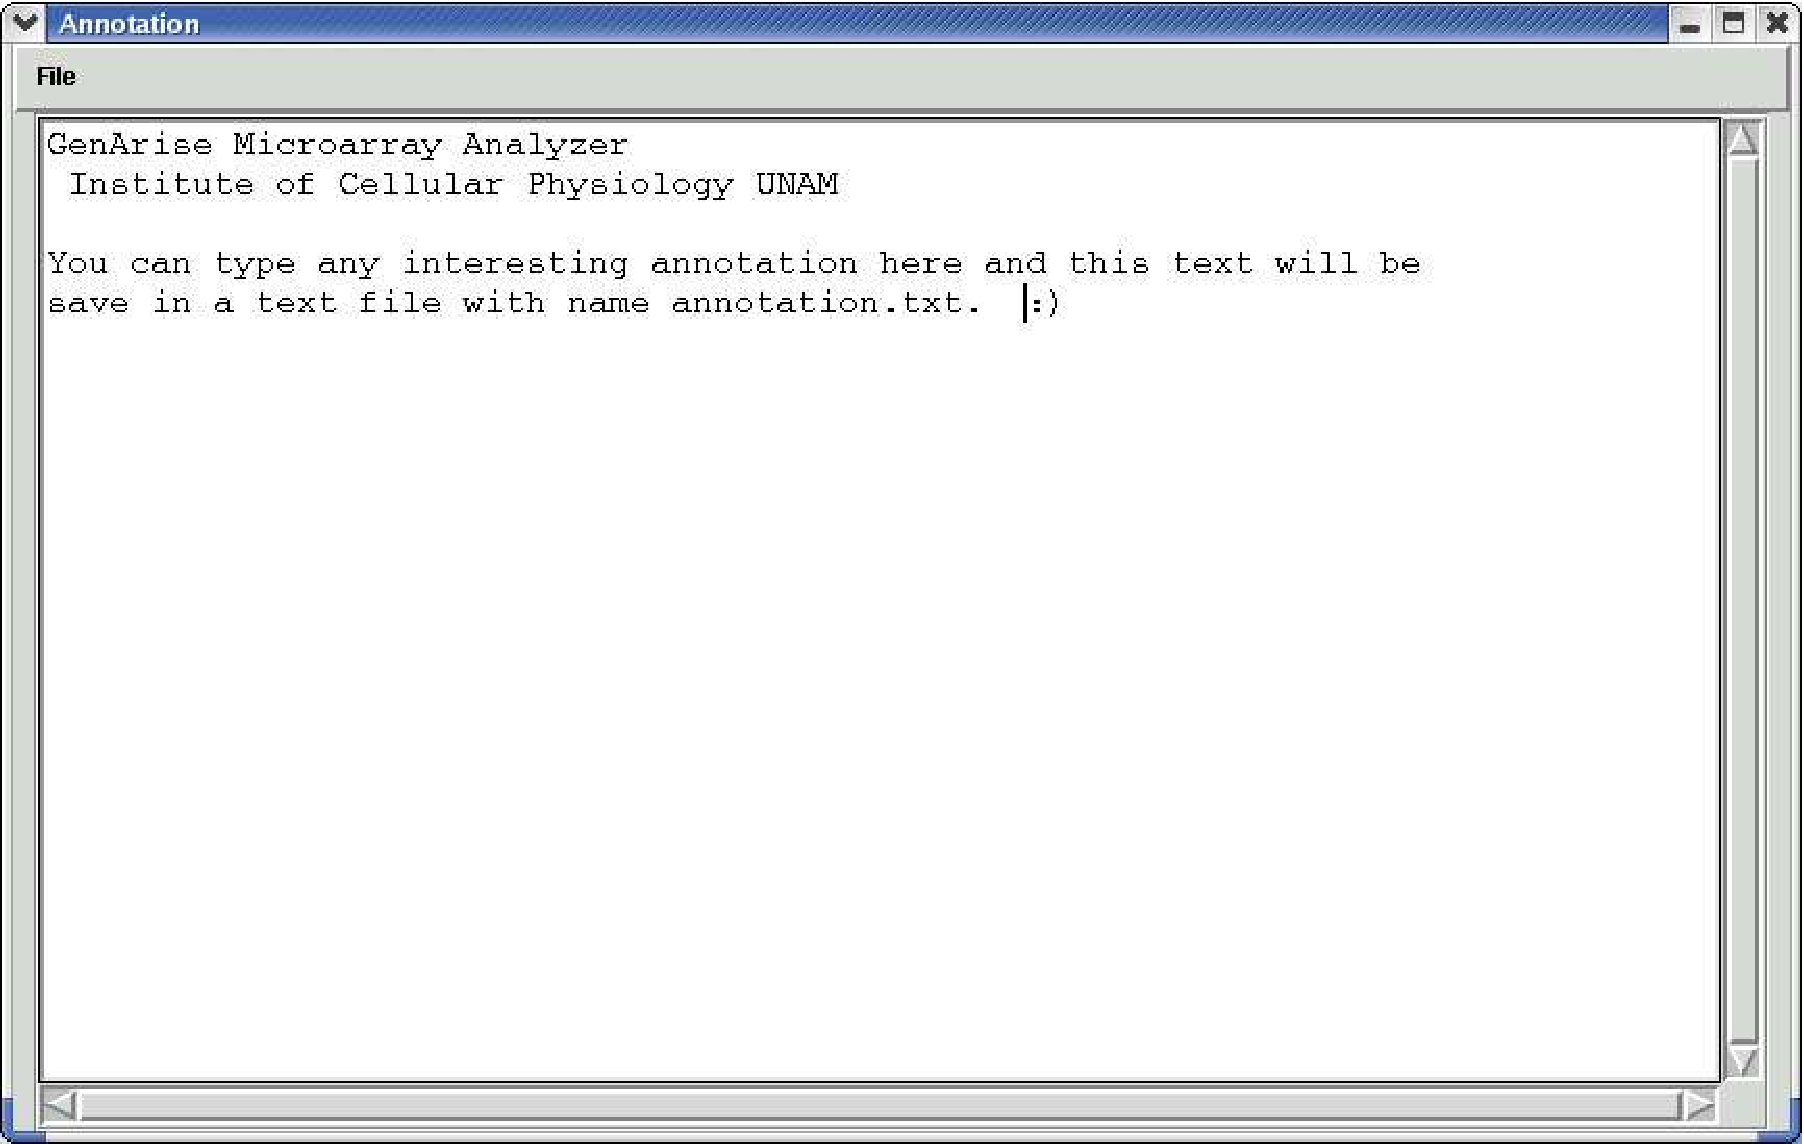
\includegraphics[scale= 0.3]{./images/annotation.pdf}\\
\caption{An Editor for annotations\label{fig6}}
\end{center}
\end{figure}

At this moment we can begin the analysis by clicking on the menu Analyze that will display a dialog box like the next one:
\begin{figure}[h]
\begin{center}

\includegraphics[scale= 0.3]{./images/wizarddialog.pdf}\\
\caption{Asking dialog box.\label{fig7}}
\end{center}
\end{figure}

By clicking \textbf{Yes }the program makes the operations in a sequential order that follows the Cellular Physilogy Institute UNAM; these operations are: background correction, loess normalization, filter, duplicate elimination. Once this analysis end we see the next window.

\begin{figure}[h]
\begin{center}
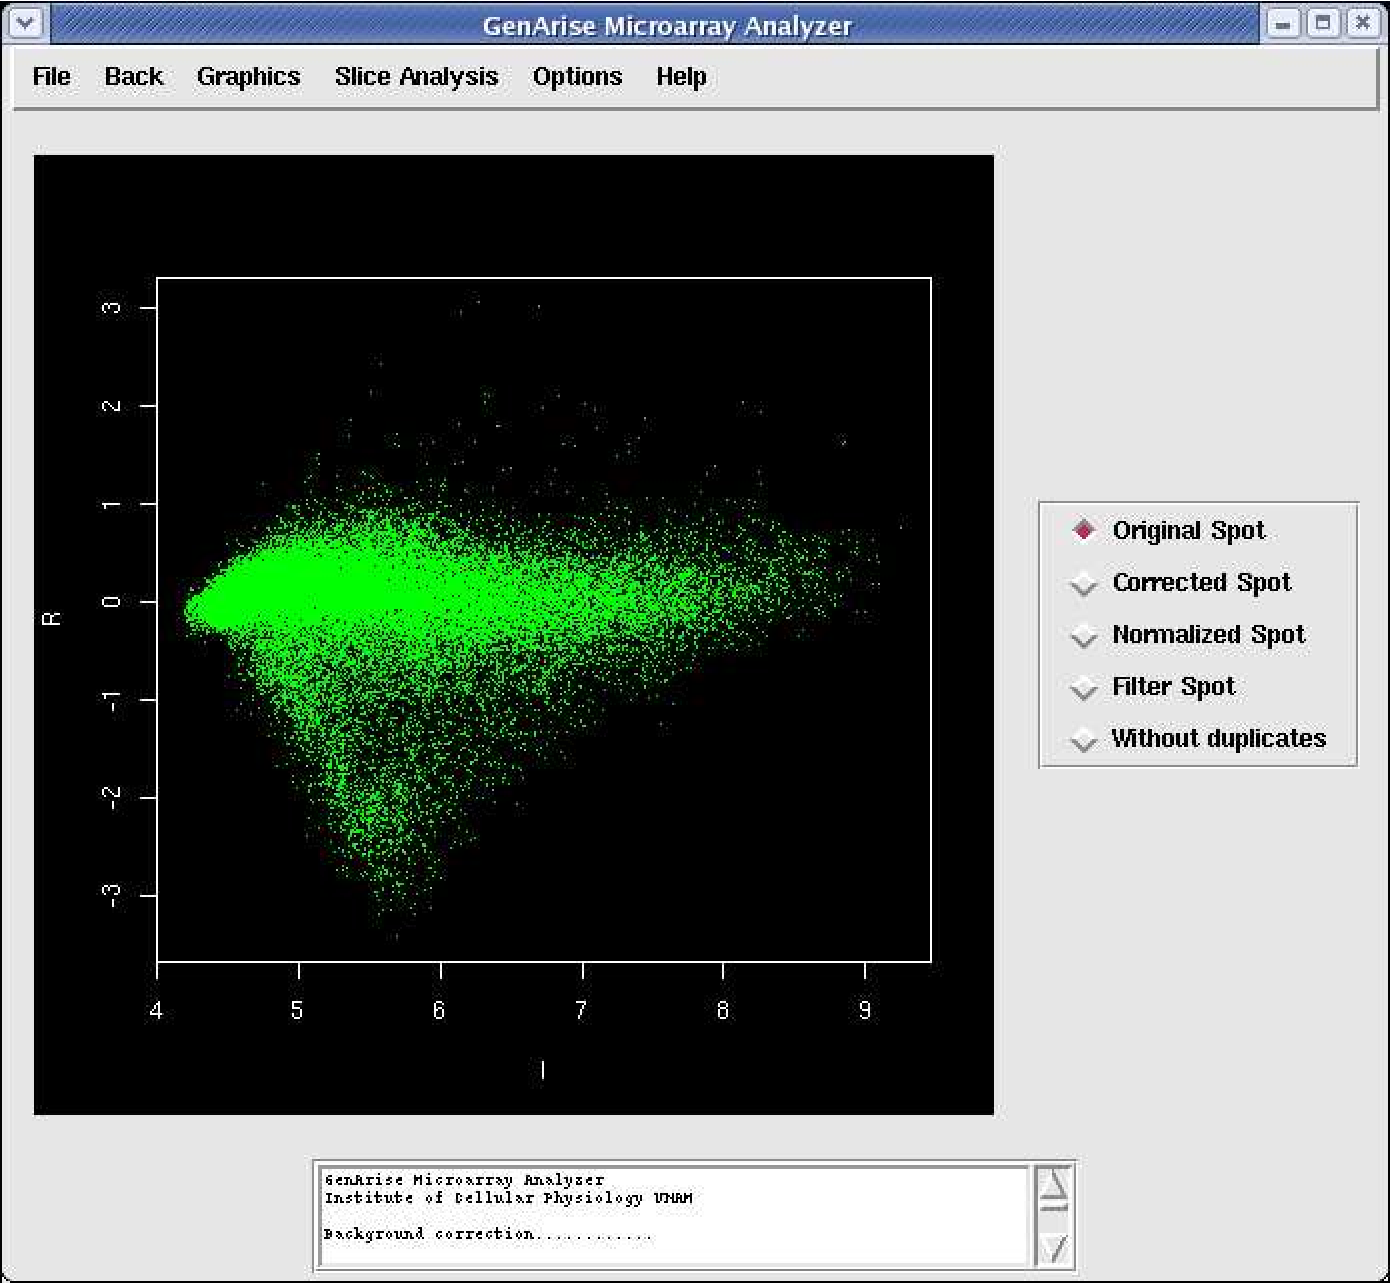
\includegraphics[scale= 0.3]{./images/wizardOriginal.pdf}\\
\caption{Text area while analisis.. \label{fig8}}
\end{center}
\end{figure}

This windows shows the graphic obtained from the complete analysis, also shows five options where we can select the original-experiment graphic and after each oparation; for example after select the option \textbf{Normalized Spot} the next result is shown:
\begin{figure}[h]
\begin{center}
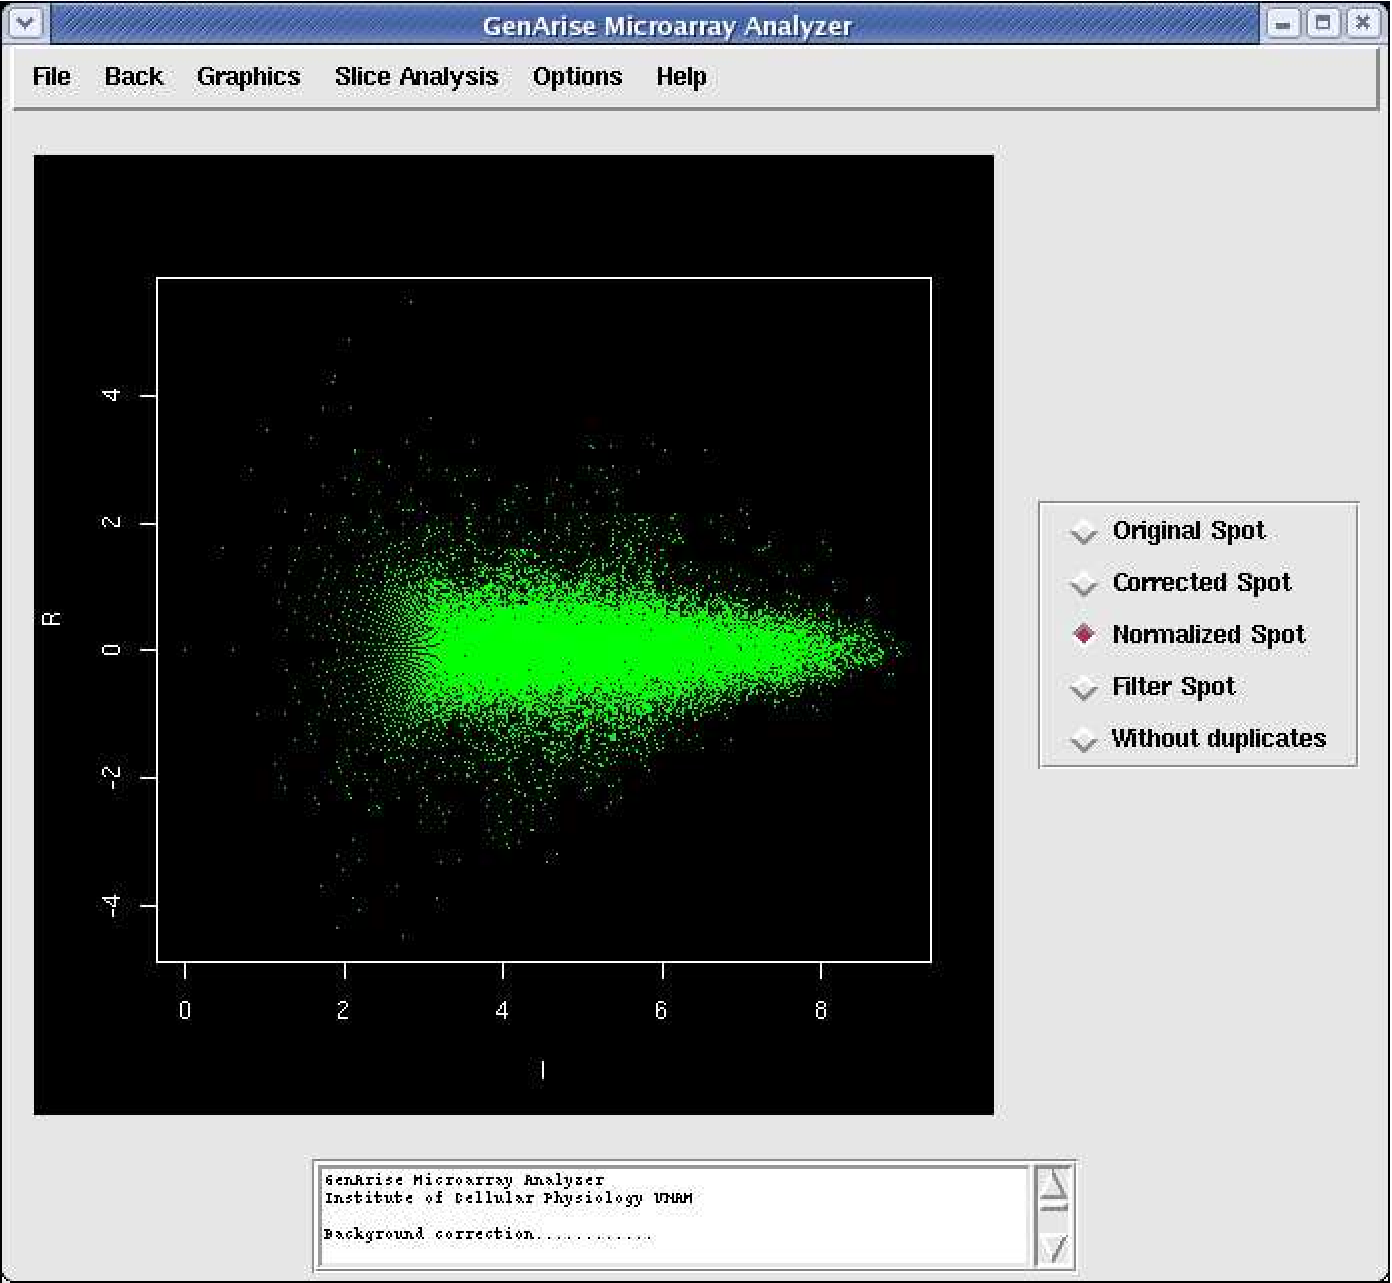
\includegraphics[scale= 0.3]{./images/wizardNorm.pdf}\\
\caption{You can select any step of this analisis for preview \label{fig9}}
\end{center}
\end{figure}

There are a text area in the lower side of the window where we can find the operations done and their values.When we follow the wizard the default values are employed in the operations, in this case, for the filter operation we take as keywords the words \textbf{empty, 0 and blank }. The threshold value is \textbf{max(max(Cy3),max(Cy5))* 0.01.}. We use the grid normalization.\\
The menu \textbf{Graphics} allow us change the type of the graphic that is displayed. The options are:  \textbf{Cy3 vs Cy5, R vs I } and \textbf{M vs A}, if you select \textbf{Cy3 vs Cy3} as shown the next figure.
\begin{figure}
\begin{center}
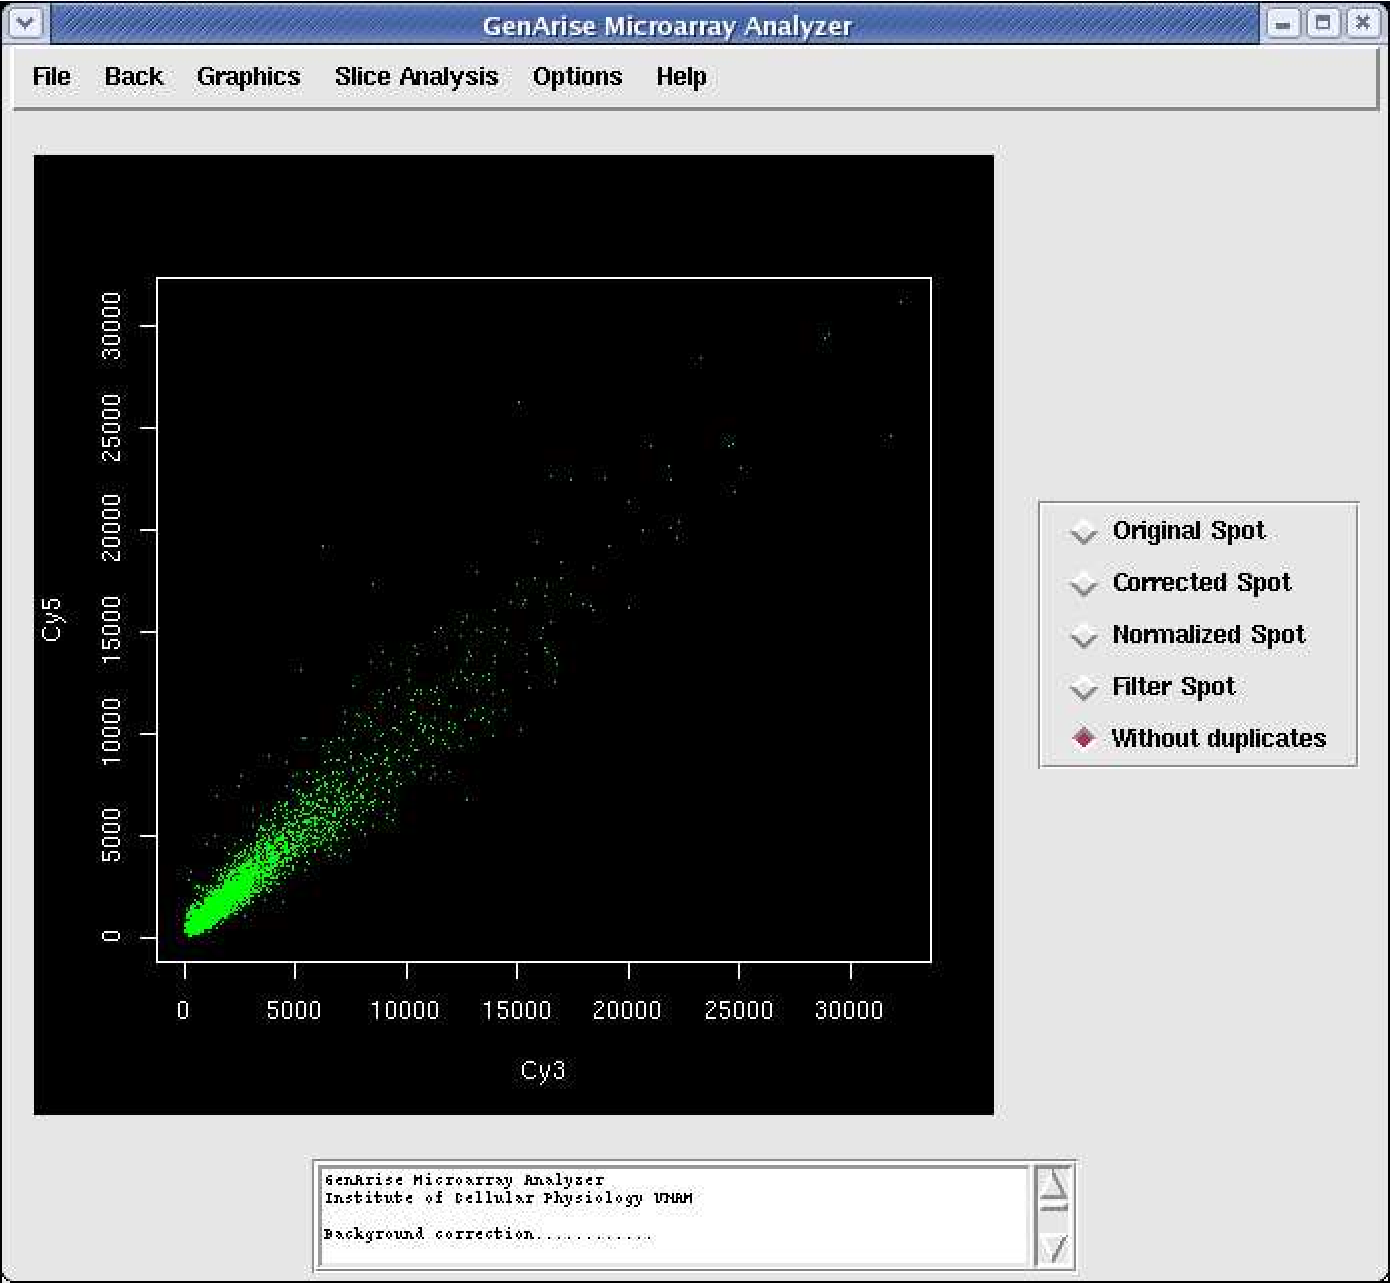
\includegraphics[scale= 0.3]{./images/nodupsCy3vsCy5.pdf}
\caption{}
\end{center}
\end{figure}

At the end, we find one file for each done operation, as well as for each graphic, in the directory where are the result files of our project.\\

Let see what happen if we decide don't follow the wizard. In this case only the original-experiment graphic is displayed as shown the next image.


\begin{center}
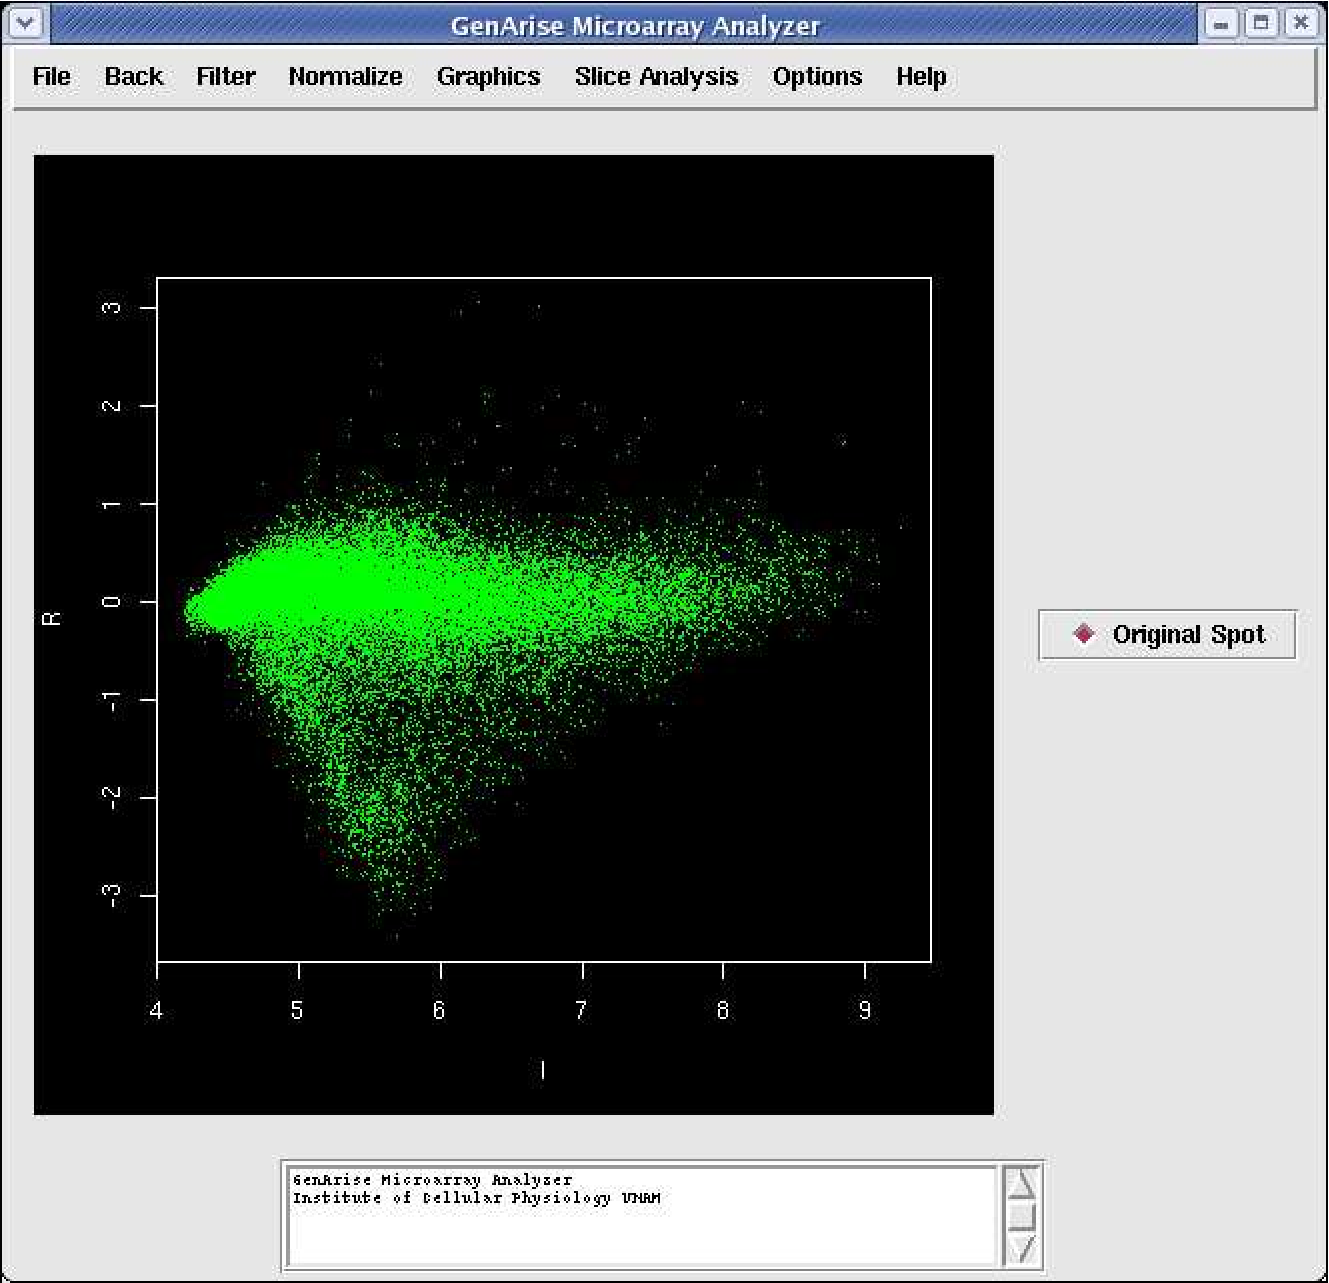
\includegraphics[scale= 0.3]{./images/original.pdf}
\end{center}

In the menu bar we should select the operations we wish the program make in the desired order, once an operation is made  a new radiobutton appears in the right side of the window with which we can see the graphic's results obtained with that operation, is important to note that the operations is realiced on the selected spot. If we wish to make a sequential analysis we must take care on the selected spot. The operations the program make when we decide follow the wizard are the same that we can find in the menu\textbf{Options}.\\

\end{document}
